\chapter{روش عددی}
\label{ch:fasl3}
در این قسمت روش عددی استفاده شده برای حل معادلات را شرح خواهیم داد.
%----------------------------------------------------------------------------------------ی
%----------------------------------------------------------------------------------------ی
%                                      قسمت اوّل: بدون بعد سازی معادلات
%----------------------------------------------------------------------------------------ی
%----------------------------------------------------------------------------------------ی
\section{بدون بعد سازی معادلات}
ابتدا برای ساده‌تر شدن کار با معادلات آن‌ها را بی‌بعد می‌سازیم، به همین منظور مقادیر مرجع طول $L^*$، فشار $P^*$، زمان $T^*$، تراوایی مطلق $K^*$ و سرعت $u^*$ را تعریف می‌کنیم. حال می‌توانیم پارامتر‌های بدون بعد را به صورت معادله \ref‌فر{eq:3dim1} تعریف کنیم:
\begin{equation}
\label{eq:3dim1}
\tilde{x}=\frac{x}{L^*} \quad
\tilde{y}=\frac{y}{L^*} \quad
\tilde{h}=\frac{h}{L^*} \quad
\tilde{\varphi}_\alpha=\frac{\varphi_\alpha}{P^*} \quad 
\tilde{t}=\frac{t}{T^*} \quad 
\tilde{\textbf{K}}=\frac{\textbf{K}}{K^*} \quad
\tilde{u}=\frac{u}{u^*}
\end{equation}

حال با جایگذاری مقادیر بی‌بعد در معادلات \ref‌فر{eq:2phic}، \ref‌فر{eq:2comp1}--\ref‌فر{eq:2comp4} خواهیم داشت:
\begin{align}
\label{eq:3dim2}
&\tilde{\nabla}\cdot\left[
\left(k_{rw}+\frac{k_{ro}}{\mathcal{M}}\right)\tilde{\textbf{K}}\tilde{\nabla}\tilde{\varphi}_w +
\frac{k_{ro}}{\mathcal{M}}\tilde{\textbf{K}}\tilde{\nabla}\tilde{\varphi}_c \right] = 0\\
\label{eq:3dim3}
&\mathcal{N}\tilde{\phi}\frac{\partial S}{\partial \tilde{t} } - \tilde\nabla\cdot
\left[ k_{rw}\tilde{\textbf{K}}\tilde{\nabla}\tilde{\varphi_w} \right] = 0 \\
\label{eq:3dim4}
&\tilde{u} = -\frac{1}{\mathcal{P}} \cdot \left[
\left(k_{rw}+\frac{k_{ro}}{\mathcal{M}}\right)\tilde{\textbf{K}}\tilde{\nabla}\tilde{\varphi}_w +
\frac{k_{ro}}{\mathcal{M}}\tilde{\textbf{K}}\tilde{\nabla}\tilde{\varphi}_c \right] \\
\label{eq:3dim5}
&\tilde{u}_w =-\frac{1}{\mathcal{P}} \cdot 
k_{rw}\tilde{\textbf{K}}\tilde{\nabla}\tilde{\varphi_w} \\
\label{eq:3dim6}
&\tilde{\varphi_c} = \tilde{P_d}J(S) + \mathcal{G} \tilde{h} 
\end{align}

پارامتر‌های بدون بعد
$\tilde{\phi}$، $\mathcal{M}$، $\mathcal{N}$، $\mathcal{P} $ و $\mathcal{G}$
به صورت زیر تعریف می‌شوند:
\begin{equation}
\label{eq:3dim7}
\tilde{\phi}=\beta\phi \quad
\mathcal{M}= \frac{\mu_o}{\mu_w}\quad
\mathcal{N}= \frac{L^*\mu_w}{P^* K^*} \cdot \frac{L^*}{T^*} \quad
\mathcal{P}= \frac{L^*\mu_w}{P^* K^*} \cdot u^* \quad
\mathcal{G}= \frac{(\varrho_o - \varrho_w) g L^*}{P^*} 
\end{equation}

از این‌جا به بعد دیگر بالاوند مد را برای پارامتر‌های بدون بعد استفاده نخواهیم کرد، به زبان ریاضی:  
$(.) \doteq \tilde{(.)}$.
معادلات \ref‌فر{eq:3dim2}--\ref‌فر{eq:3dim6} اساس کار ما را تشکیل خواهند داد و برای تعریف یک مسئله کافی است پارامتر‌های $\tilde{\phi}$، $\mathcal{M}$، $\mathcal{N}$، $\mathcal{P} $ و $\mathcal{G}$، هندسه با طول بی‌بعد و شرایط مرزی (حالت بدون بعد معادلات \ref‌فر{eq:2bndout}) داده شوند.
%----------------------------------------------------------------------------------------ی
%----------------------------------------------------------------------------------------ی
%                                      قسمت دوم: مش محاسباتی
%----------------------------------------------------------------------------------------ی
%----------------------------------------------------------------------------------------ی
\section{مش مورد نیاز}
برای حل معادلات \ref‌فر{eq:3dim2}--\ref‌فر{eq:3dim6}، اولین قدم مش زدن هندسه است. مش مورد نیاز باید دو شرط مهم را داشته باشد:
\begin{tight_enumerate}
\item اضلاع المان‌ها مرز محیط‌ها و ترک‌ها را قطع نکنند، یعنی نود‌ها روی مرز نواحی و روی ترک‌ها قرار گیرند\footnote{Conforming Mesh}.
\item مش از المان‌های مثلثی، چهار‌ضلعی‌ و خطی تشکیل شده باشد و المان‌های مثلثی و چهارضلعی متعلق به نواحی ماتریس و المان‌های خطی مربوط به نواحی ترک باشند.
\end{tight_enumerate}
در شکل \ref{fig:3mesh} یک نمونه مش مناسب برای شبیه‌سازی عددی را مشاهده می‌کنید. در این مش خطوط نازک المان‌های ماتریس و خطوط کلفت المان ترک یا مرز نواحی ماتریس را نشان می‌دهند.

\begin{figure}
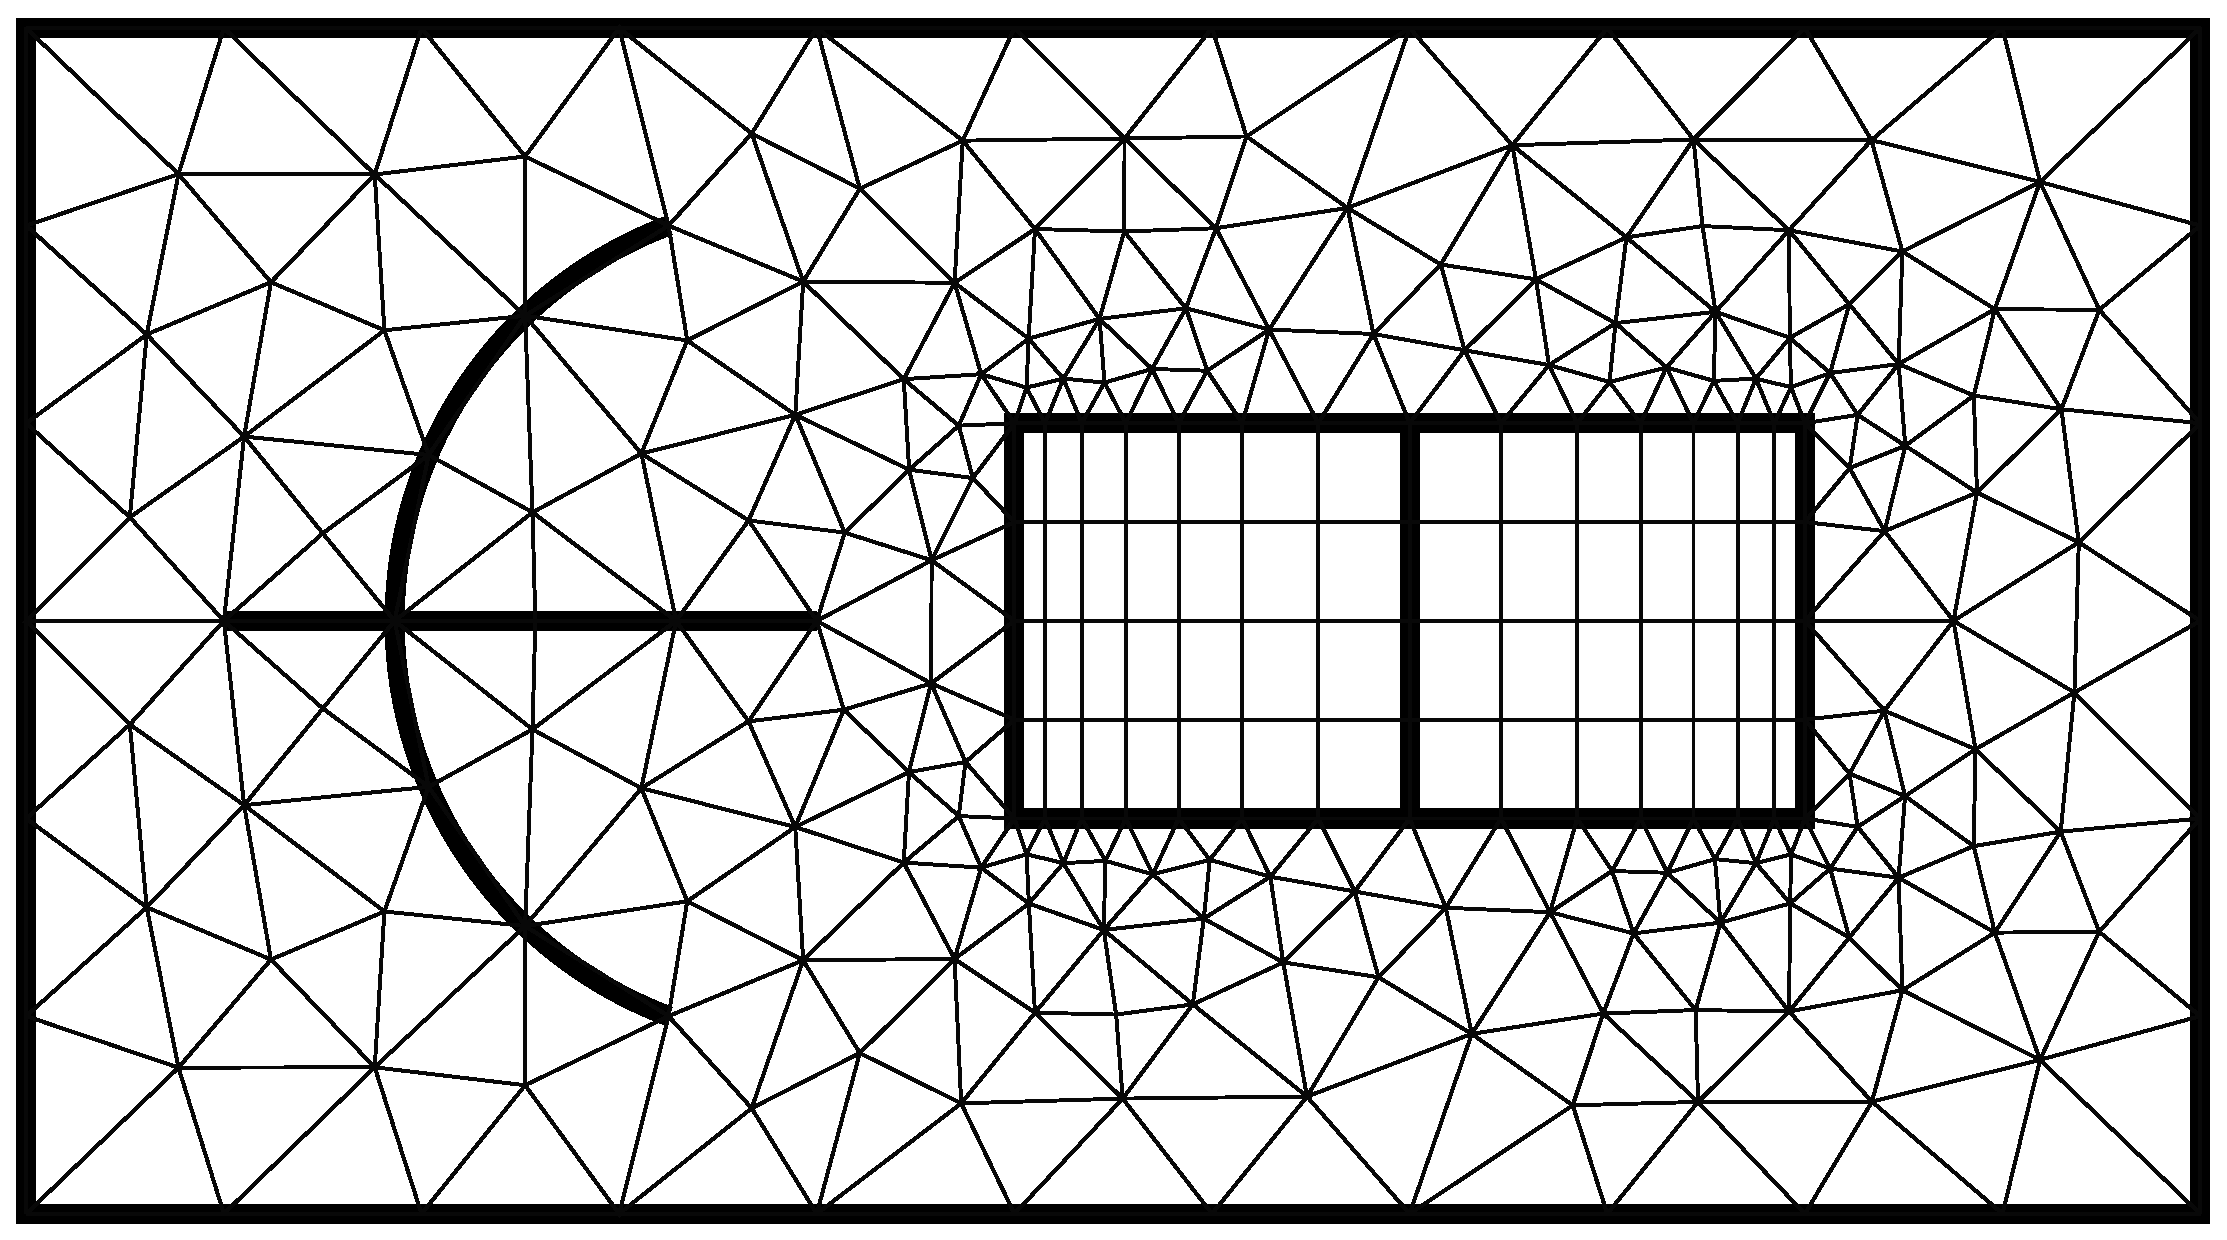
\includegraphics[width=.6\textwidth,center]{numeric-mesh.eps}
\caption{مش مناسب برای شبیه‌سازی عددی}
\label{fig:3mesh}
\end{figure}

%----------------------------------------------------------------------------------------ی
%----------------------------------------------------------------------------------------ی
%                                      قسمت سوم: نوتاسیون
%----------------------------------------------------------------------------------------ی
%----------------------------------------------------------------------------------------ی
\section{معرفی نوتاسیون استفاده شده در روش عددی}
در این قسمت نوتاسیون مورد نیاز برای بیان روش عددی را بیان خواهیم کرد. به همین منظور در شکل \ref{fig:3not} یک نود به نام $i$ یا $v_i$ و المان‌ها و نود‌های اطراف آن نمایش داده شده‌اند. همانطور که مشاهده می‌کنید امکان دارد که اطراف یک نود المان‌های ترک مثل المان $C$ یا $e_C$ نیز وجود داشته باشند. علاوه بر نمایش نام‌گذاری المان‌ها و نود‌ها در شکل \ref{fig:3not-mesh}، در شکل \ref{fig:3not-geo} تعدادی نقطه مهم از جمله وسط اضلاعی که نود $v_i$ عضوی از آنهاست مثل $\frac{ij}{2}$ و مراکز هندسی المان‌ها مثل $G_B$ نمایش داده شده‌اند. 

\begin{figure}
\begin{subfigure}{0.5\textwidth}
\includegraphics[width=.95\linewidth,center]{numeric-notation-geo.jpg} 
\caption{نقاط کمکی برای معرفی حجم کنترل و بردارها}
\label{fig:3not-geo}
\end{subfigure}
\begin{subfigure}{0.5\textwidth}
\includegraphics[width=.95\linewidth,center]{numeric-notation-mesh.jpg} 
\caption{اجزای اصلی مش}
\label{fig:3not-mesh}
\end{subfigure}

\caption{مثالی از یک نود به نام $v_i$ و اجزای اطرافش}
\label{fig:3not}
\end{figure}

اولین مفهوم مهم در مش اضلاع هندسی\footnote{Edge} هستند. به اضلاع المان‌ها، اضلاع هندسی گفته می‌شوند. برای مثال در شکل \ref{fig:3not} خطوط $ij$ یا $ik$ اضلاع هندسی هستند. مفهوم مهم دیگر احجام کنترل هستند. با روشی که ذکر خواهیم کرد متناظر با هر نود یک حجم کنترل خواهیم ساخت: نقاط وسط اضلاع هندسی اطراف هر نود را به مرکز حجم المان متناظرش متصل می‌کنیم. چند ضلعی حاصله حجم کنترل متناظر با نود مذکور خواهد بود. برای مثال در شکل \ref{fig:3not} حجم کنترل متناظر با نود $i$، چند ضلعی 
$G_BG_CG_D\frac{io}{2}G_E\frac{ij}{2}G_A\frac{ik}{2}$
است. مفهوم بعدی اضلاع دوگانه\footnote{Dual-edge} است. به هر یک از اضلاع احجام کنترل یک ضلع دوگانه می‌گوییم. با دقت در شکل \ref{fig:3not} می‌توان مشاهده کرد که متناظر با هر ضلع هندسی به تعداد المان‌هایی که این ضلع هندسی عضو آن‌هاست، ضلع دوگانه وجود دارد. یعنی به ازای هر ضلع هندسی و هر المان یک ضلع دوگانه وجود دارد. برای مثال ضلع دوگانه 
$G_E\frac{ij}{2}$
متناظر با ضلع هندسی $ij$ در المان $E$ است و یا  پاره‌خطی به طول $e$(ضخامت المان ترک $C$) که از $G_C$ می‌گذرد، ضلع دوگانه متناظر با ضلع هندسی $im$ در المان ترک $C$ می‌باشد.

مفهوم مهم دیگر المثنی‌ها\footnote{Duplicates} هستند. از بخش \ref{ch:253} می‌دانیم که در هر نود که روی مرز چند ناحیه قرار گیرد، چند مقدار اشباع باید ذخیره شود. به همین منظور مفهومی به نام المثنی‌ها را معرفی می‌کنیم. به ازای هر نود در مش به تعداد نواحی احاطه کننده آن، المثنی وجود خواهد داشت. المثنی‌ها اشیاء فرضی هستند که مقادیری مثل اشباع را به آن‌ها نسبت خواهیم داد. برای مثال در شکل \ref{fig:3not} سه ناحیه مختلف (دو ناحیه ماتریس و یک ناحیه ترک) نود $i$ را احاطه کرده‌اند. لذا سه المثنی متناظر با این نود وجود خواهد داشت. در این شکل این سه المثنی را
$d_1$، $d_2$ و $d_3$
نامیده‌ایم. مطابق دستورالعملی که در فصل \ref{ch:fasl2} بیان شد، یکی از این المثنی‌ها ارباب و بقیه برده‌ خواهند بود و مقدار اشباع برده‌ها وابسته به مقدار اشباع در ارباب خواهد بود. برخلاف اشباع، مقادیری مثل پتانسیل آب $\varphi_w$ بنابر معادله \ref‌فر{eq:2bndin} به نواحی بستگی ندارند، لذا به نود‌ها نسبت داده ‌می‌شوند.

دیگر مفاهیم مورد نیاز، به همراه مثالی از شکل \ref{fig:3not} به شرح زیر هستند:  
\begin{tight_itemize}
\item[$v_i$]
نود شماره $i$
\item[$e_i$]
المان شماره $i$
\item[$B_i$]
حجم کنترل متناظر با نود شماره $i$  
\item[$B_i^j$]
قسمتی از حجم کنترل متناظر با نود شماره $i$ که در المان $j$ قرار دارد. برای مثال $B_i^A$ چهار ضلعی
$v_i\frac{ij}{2}G_A\frac{ik}{2}$
می‌باشد.  
\item[$n_{ij}^k$]
بردار یکه عمود بر ضلع دو‌گانه متناظر با ضلع هندسی $ij$ در المان $k$ که جهت آن از $i$ به سمت $j$ است. برای مثال 
$n_{im}^C$
برداری یکه در راستای خط $v_iv_m$ از $v_i$ به سمت $v_m$ می‌باشد و یا 
$n_{im}^B$
برداری یکه عمود بر خط $G_CG_B$ از $v_i$ به سمت $v_m$ می‌باشد. 
\item[$g_{ij}^k$]
نقطه وسط ضلع دو‌گانه متناظر با ضلع هندسی $ij$ در المان $k$. برای مثال  
$g_{im}^C$
نقطه $G_C$ و یا 
$g_{im}^B$
نقطه وسط پاره‌خط $G_CG_B$ می‌باشد.  
\item[$l_{ij}^k$]
طول ضلع دو‌گانه متناظر با ضلع هندسی $ij$ در المان $k$. 
\item[\lr{NE}]
تعداد المان‌های موجود در کل مش. 
\item[\lr{NV}]
تعداد نود‌های موجود در کل مش. 
\item[$N_i$]
تعداد المثنی‌های متناظر با نود $v_i$. برای مثال $N_i=3$. 
\item[$N^i$]
تعداد نود‌های عضو المان $e^i$. این مقدار برای المان‌های ترک، مثلث و چهارضلعی به ترتیب برابر ۲، ۳ و ۴ می‌باشد. 
\item[$d_i$]
المثنی شماره $i$
\item[$d_i^k$]
المثنی متناظر با نود $v_i$ در المان $e_k$. برای مثال:
$d_i^A=d_i^B=d_1$، $d_i^D=d_i^E=d_3$ و $d_i^C = d_2$ 
\item[$d_i^*$]
 المثنی ارباب متناظر با نود $v_i$ 
\item[$\alpha(v_i)$]
مجموعه نود‌های اطراف نود $v_i$ و خودش. برای مثال:
$\alpha(v_i) = \left\{ v_i, v_j, v_k, v_l, v_m, v_n, v_o \right\}$ .
\item[$\theta(v_i)$]
 مجموعه المان‌های اطراف نود $v_i$. برای مثال:
$\theta(v_i) = \left\{ e_A, e_B, e_C, e_D, e_E \right\}$ . 
\item[$\sigma(e_i)$]
 مجموعه نود‌های عضو المان $e_i$. برای مثال:
$\theta(e_B) = \left\{ v_m, v_i, v_k, v_l \right\}$ و یا $\theta(e_C) = \left\{ v_i, v_m \right\}$ 
\item[$\eta(v_i,e_j)$]
مجموعه نود‌های عضو المان $e_j$ که با نود $v_i$ ضلع هندسی مشترک دارند. برای مثال:\\
$\eta(v_i,e_B) = \left\{ v_k, v_m \right\}$ و یا $\eta(v_i,e_C) = \left\{  v_m \right\}$ 
\item[$\gamma(v_i)$]
 مجموعه المثنی‌های مرتبط با نود $v_i$. برای مثال:
$\gamma(v_i) = \left\{ d_1, d_2, d_3 \right\}$ 
\item[$\textbf{K}^i$]
تراوایی مطلق متناظر با المان $e_i$ 
\item[$\phi^i$]
تخلخل متناظر با المان $e_i$ 
\item[$\chi|_{vi}$]
 متغیر $\chi$ ذخیره شده در نود $v_i$. تنها متغیری که متناظر با نودهاست و می‌تواند به جای $\chi$ قرار بگیرد $\varphi_w$ می‌باشد. 
\item[$\chi|_{di}$]
 متغیر $\chi$ ذخیره شده در المثنی $d_i$. متغیرهای
$S$، $k_{rw}$، $k_{ro}$ و $\varphi_c$
می‌توانند به جای $\chi$ قرار گیرند. 
\item[$\chi|_{g_{ij}^k}$]
مقدار متغیر $\chi$ در نقطه $g_{ij}^k$ که به کمک روش \text‌لاتین{upwind} و از درون‌یابی مقادیر $\chi|_{di}$ پیدا می‌شود. متغیرهای
$k_{rw}$ و $k_{ro}$
می‌توانند به جای $\chi$ قرار گیرند. 
\item[$\nabla\chi|_{g_{ij}^k}$]
مقدار گرادیان متغیر $\chi$ در نقطه $g_{ij}^k$ که به کمک مقادیر $\chi|_{di}$ و یا $\chi|_{vi}$ پیدا می‌شود. متغیرهای
$\varphi_w$ و $\varphi_c$
می‌توانند به جای $\chi$ قرار گیرند. 
\item[$\vec{X}_{v_i}$]
مختصات نود $v_i$
\end{tight_itemize}

قبل از رفتن به بخش بعدی نحوه محاسبه
 $k_{ro}|_{g_{ij}^k}$، $k_{rw}|_{g_{ij}^k}$،  $\nabla\varphi_w|_{g_{ij}^k}$ و $\nabla\varphi_c|_{g_{ij}^k}$ 
را بیان می‌کنیم. برای محاسبه $k_{ro}|_{g_{ij}^k}$ و $k_{rw}|_{g_{ij}^k}$ از روش \text‌لاتین{upwind} استفاده می‌نماییم. این روش در معادله \ref‌فر{eq:3up} بیان شده است.
\begin{equation}
\label{eq:3up}
k_{r\alpha}|_{g_{ij}^k} = 
\begin{cases}
k_{r\alpha}|_{d_i^k}	&u_\alpha \cdot n_{ij}^k \geq 0 \\
k_{r\alpha}|_{d_j^k}	&u_\alpha \cdot n_{ij}^k < 0
\end{cases}
\quad \alpha = w,o
\end{equation}
در این معادله مقادیر $u_\alpha$ باید از معادلات \ref‌فر{eq:3dim4}، \ref‌فر{eq:3dim5} محاسبه شوند.

برای محاسبه  $\nabla\varphi_\alpha|_{g_{ij}^k}$  از توابع شکل\footnote{Shape Functions} استفاده می‌کنیم. به این منظور در هر المان برای هر نود یک تابع شکل تعریف می‌کنیم: $\psi_i^k$ یعنی تابع شکل نود $v_i$ در المان $e_k$. ویژگی تابع شکل 
این است که مقدار آن در نود متناظرش باید برابر یک شود ولی در دیگر نود‌ها مقدار آن باید برابر صفر شود. به زبان ریاضی:
\begin{equation}
\label{eq:sf1}
\psi_i^k (\vec{X}_{v_j}) 
\begin{cases}
1	&i=j \\
0	&i\neq j
\end{cases}
\quad v_i,v_j \in \sigma (e_k)
\end{equation}
با تعریف توابع شکل می‌توانیم توزیع متغیر $\varphi_w$ را به صورت معادله \ref‌فر{eq:3sf2} در هر المان باز‌سازی کنیم:
\begin{equation}
\label{eq:3sf2}
\varphi_w(\vec X) = \sum_{v_j \in \sigma(e_i)} \psi_j^i(\vec X) \varphi_w|_{v_j}
\quad \vec{X} \text{  inside  }  e_i
\end{equation}

لذا با مشتق‌گیری از معادله  \ref‌فر{eq:3sf2} و قرار دادن مختصات نقاط $g_{ij}^k$ به جای $\vec X$ مقدار $\nabla\varphi_w|_{g_{ij}^k}$ محاسبه می‌شود:
\begin{equation}
\label{eq:3sf3}
\nabla \varphi_w|_{g_{ij}^k} = \sum_{v_l \in \sigma(e_k)} \nabla \psi_l^k(\vec X_{g_{ij}^k}) \varphi_w|_{v_j}
\quad  v_i,v_j \in  \sigma(e_i)
\end{equation} 

به طریقه مشابه برای محاسبه گرادیان پتانسیل مویینگی داریم:
\begin{equation}
\label{eq:3sf4}
\nabla \varphi_c|_{g_{ij}^k} = \sum_{v_l \in \sigma(e_k)} \nabla \psi_l^k(\vec X_{g_{ij}^k}) \varphi_c|_{d_j^k}
\quad  v_i,v_j \in  \sigma(e_i)
\end{equation} 

تنها تفاوت معادلات  \ref‌فر{eq:3sf3} و  \ref‌فر{eq:3sf4} این است که مقادیر پتانسیل آب در نود‌ها ذخیره می‌شوند ولی مقادیر پتانسیل مویینگی در المثنی‌ها ذخیره می‌شوند.
%----------------------------------------------------------------------------------------ی
%----------------------------------------------------------------------------------------ی
%                                      قسمت چهارم: روش IMPES
%----------------------------------------------------------------------------------------ی
%----------------------------------------------------------------------------------------ی
\section{روش \text‌لاتین{IMPES}}
در این قسمت توضیح خواهیم داد که در هر گام زمانی چه معادلاتی باید حل شوند و مجهولات معادلات چه هستند.

هدف در این پروژه پیدا کردن مقادیر $S|_{di}$ و $\varphi|_{vi}$ در هر گام زمانی می‌باشد، اما همانطور که در  بخش  \ref{ch:253} نشان دادیم، مقادیر
 $S|_{d_i} \quad d_i\in\gamma(v_j)$
 مستقل از یکدیگر نیستند و همگی تابع  $S|_{d_j^*}$  هستند. لذا مجهولات خود را دو بردار 
$\vec{\Phi}^k$ و $\vec{S}^k$
تعریف می‌کنیم، که به ترتیب مقادیر $\varphi|_{v_i}$ و $S|_{d_i^*}$ را در گام زمانی $k$ام نشان می‌دهند. طول هر دو بردار نیز برابر \text‌لاتین{NV} می‌باشد.

فرض کنید در گام زمانی $k$ مقدار $\vec{S}^k$ مشخص است. روش \text‌لاتین{IMPES} برای پیدا کردن دو بردار 
$\vec{\Phi}^k$ و $\vec{S}^{k+1}$
فرآیند ذیل را پیشنهاد می‌دهد:
\begin{tight_enumerate}
\item با گسسته سازی معادله \ref‌فر{eq:3dim2} مقدار $\vec{\Phi}^k$ را محاسبه کنید. به این منظور باید دستگاهی به صورت زیر را حل نمایید:
\begin{equation}
\label{eq:3impes1}
\begin{aligned}
&\textbf{A}_G \vec{\Phi}^k = \vec{\mathcal{B}}_G \\
& \textbf{A}_G = \textbf{A}_G(\vec{S}^k, \Gamma_{\varphi N}, \Gamma_{\varphi D})\\
& \vec{\mathcal{B}}_G = \vec{\mathcal{B}}_G(\vec{S}^k, \Gamma_{\varphi N}, \Gamma_{\varphi D}) 
\end{aligned}
\end{equation}
در واقع نام فشار ضمنی به این خاطر به این روش داده شده‌است که پتانسیل آب در معادله \ref‌فر{eq:3impes1} به صورت ضمنی حل می‌شود. همانطور که مشاهده می‌کنید، طرف چپ و راست این معادله صرفاً تابعی از اشباع در بازه زمانی $k$ و شرایط مرزی پتانسیل آب هستند، لذا معادله کاملاً خطی خواهد بود.
\item سپس با گسسته سازی معادله \ref‌فر{eq:3dim3} مقدار $\vec{S}^{k+1}$ را محاسبه کنید. به این منظور باید معادله‌ای به صورت زیر را حل نمایید:
\begin{equation}
\label{eq:3impes2}
\begin{aligned}
&\frac{1}{\triangle t} \vec{\mathcal C}_G \cdot \triangle\vec S^k = \vec{\mathcal{F}}_G \\
&\vec{S}^{k+1} =  \vec{S}^{k} + \triangle\vec{S}^{k} \\
& \vec{\mathcal C}_G = \vec{\mathcal C}_G(\vec{S}^k,\vec{\Phi}^k)\\
& \vec{\mathcal F }_G = \vec{\mathcal{F}}_G(\vec{S}^k,\vec{\Phi}^k, \Gamma_{SN}, \Gamma_{SD}) 
\end{aligned}
\end{equation}
در این معادله اشباع در گام زمانی $k+1$ به صورت کاملاً صریح حل شده است و برخلاف معادله \ref‌فر{eq:3impes1} دیگر یک دستگاه نیست. همین عمل است که باعث خطی شدن معادله می‌شود، امّا برای همگرا شدن پاسخ‌ها باید گام زمانی کوچک انتخاب شود. 
\end{tight_enumerate}

در قسمت بعدی نشان خواهیم داد که بردار‌های 
$\vec{\mathcal B}_G$، $\vec{\mathcal C}_G$، $\vec{\mathcal F}_G$ و ماتریس $\textbf{A}_G$
در هر گام زمانی چگونه محاسبه خواهند شد.
%----------------------------------------------------------------------------------------ی
%----------------------------------------------------------------------------------------ی
%                                      قسمت پنجم:۳۵ معادله حجم محدود
%----------------------------------------------------------------------------------------ی
%----------------------------------------------------------------------------------------ی
\section{معادله حجم محدود}
\label{ch:35}
در این قسمت روش حجم محدود را برای محاسبه بردار‌های 
$\vec{\mathcal B}_G$، $\vec{\mathcal C}_G$، $\vec{\mathcal F}_G$ و ماتریس $\textbf{A}_G$
معرفی خواهیم کرد. روش حجم محدود استفاده شده \text‌لاتین{CVFEM}\footnote{Control Volume Finite Element} نام دارد و اوّلین بار در \cite{baliga} برای حل معادله \text‌لاتین{advection-diffusion} به کار رفته‌است. نحوه تعمیم این روش برای حل معادلات جریان دوفازی در محیط متخلخل از  \cite{mont1} گرفته شده‌است. 
%--------------------------------------------۳۵۱ معادله پتانسیل------------------------------ی
\subsection{معادله پتانسیل}
ابتدا نحوه ایجاد معادله \ref‌فر{eq:3impes1} را از معادله \ref‌فر{eq:3dim2} بیان خواهیم کرد. به این منظور ابتدا از معادله \ref‌فر{eq:3dim2} در هر حجم کنترل $B_i$ انتگرل می‌گیریم و از قضیه دیورژانس برای انتقال انتگرال‌های حجمی به مرز استفاده می‌کنیم:
\begin{equation}
\label{eq:3fvmp1}
\int_{\partial B_i} \left[ 
\left( k_{rw}+\frac{k_{ro}}{\mathcal{M}}\right) \textbf{K} \nabla \varphi_w + 
\left(\frac{k_{ro}}{\mathcal{M}}\right) \textbf{K} \nabla \varphi_c
\right] \cdot \vec{n} d\Gamma
= 0
\quad i=1,\ldots,\text{NV}
\end{equation}

برای بیان تقریب عددی معادله \ref‌فر{eq:3fvmp1} ابتدا تقریب عددی کل شار عبوری از نود $v_i$ به سمت نود $v_j$ در المان $e_k$ را به صورت زیر تعریف می‌کنیم:
\begin{equation}
\label{eq:3fvmp2}
\begin{aligned}
-\text{TFlux}_{ij}^k 
&=
\left.\left( k_{rw}+\frac{k_{ro}}{\mathcal{M}}\right)\right|_{g_{ij}^k} \textbf{K}^k \nabla \varphi_w|_{g_{ij}^k}
\cdot (ln)_{ij}^k +
\left.\left( \frac{k_{ro}}{\mathcal{M}}\right)\right|_{g_{ij}^k} \textbf{K}^k \nabla \varphi_c|_{g_{ij}^k} 
\cdot (ln)_{ij}^k \\
&= -\mathcal{P}u \cdot (l\vec{n})_{ij}^k
\qquad e_k \in \theta(v_i) \text{  and  } v_j \in \eta(v_i,e_k)
\end{aligned}
\end{equation}

از حالت اوّل برای المان‌های داخلی و از حالت دوم برای المان‌های مجازی (اعمال شروط مرزی) استفاده خواهیم کرد. حال تقریب عددی معادله \ref‌فر{eq:3fvmp1} به صورت زیر در خواهد آمد:
\begin{equation}
\label{eq:3fvmp3}
\sum_{e_k\in\theta(v_i)} \sum_{v_j\in\eta(v_i,e_k)} -\text{TFlux}_{ij}^k = 0
\quad i = 1,\ldots,\text{NV}
\end{equation}

معادله \ref‌فر{eq:3fvmp3} به این معنی است که جمع جبری کل شار ورودی و خروجی به هر حجم کنترل برابر صفر باشد. حال برای اینکه بتوان معادلات \ref‌فر{eq:3fvmp3} را به شکل دستگاه معادلات \ref‌فر{eq:3impes1} در آورد و ماتریس $\textbf{A}_G$ و بردار $\vec{\mathcal B}_G$ را از آن استخراج نمود، فرض می‌کنیم که $\text{TFlux}_{ij}^k$ در هر المان تابعی خطی از مقدار پتانسیل آب در نود‌های عضو المان باشد، یعنی:
\begin{equation}
\label{eq:3fvmp4}
\sum_{v_k\in\eta(v_j,e_i)} -\text{TFlux}_{jk}^i = \sum_{v_k\in\sigma(e_i)} a_{jk}^i \varphi_w|_{v_k} + b_j^i
\quad i = 1,\ldots,\text{NE} \text{  and  } v_j \in \sigma(e_i)
\end{equation}

حال نشان می‌دهیم که در صورت وچود مقادیر $a$ و $b$ چگونه به کمک آن‌ها ماتریس $\textbf{A}_G$ و بردار $\vec{\mathcal B}_G$ را بسازیم. خود اینکه مقادیر $a$ و $b$ را چگونه پیدا کنیم را در بخش \ref{ch:36} ذکر خواهیم کرد. اگر معادله \ref‌فر{eq:3fvmp4} را در معادله \ref‌فر{eq:3fvmp3} جایگذاری کنیم، خواهیم داشت:
\begin{equation}
\label{eq:3fvmp5}
\begin{aligned}
&\sum_{e_k\in\theta(v_i)} \sum_{v_j\in\eta(v_i,e_k)} -\text{TFlux}_{ij}^k = 0 \\
\Longrightarrow &\sum_{e_k\in\theta(v_i)} \left(\sum_{v_j\in\sigma(e_k)} \left(a_{ij}^k \varphi_w|_{v_j}\right) + b_i^k\right)= 0
\quad i = 1,\ldots,\text{NV}
\end{aligned}
\end{equation}

حال با عوض کردن ترتیب $\Sigma$ها به معادله زیر می‌رسیم:
\begin{equation}
\label{eq:3fvmp6}
\sum_{v_j\in\alpha(v_i)} \left( \sum_{e_k\in\theta(v_i)\cap\theta(v_j)} a_{ij}^k \right) \varphi_w|_{v_j} =
-\sum_{e_k\in\theta(v_i)} b_i^k 
\quad i = 1,\ldots,\text{NV}
\end{equation}

از مقایسه معادلات \ref‌فر{eq:3fvmp6} و \ref‌فر{eq:3impes1} درمی‌یابیم که:
\begin{align}
\label{eq:3fvmp7}
&\textbf{A}_{Gij} = 
\begin{cases}
	0	&v_i \not\in \alpha (v_j)\\
	\sum_{e_k\in\theta(v_i)\cap\theta(v_j)} a_{ij}^k  &v_i \in \alpha (v_j)
\end{cases} \\
\label{eq:3fvmp8}
&\vec{\mathcal B}_{Gi} = -\sum_{e_k\in\theta(v_i)} b_i^k
\end{align}

معادلات \ref‌فر{eq:3fvmp7} و \ref‌فر{eq:3fvmp8} به این معنا هستند که ماتریس‌ و بردار جهانی  $\textbf{A}_G$ و $\vec{\mathcal B}_G$ را می‌توان از اسمبل کردن ماتریس‌‌های محلّی $\textbf{A}^k$ و بردارهای محلّی $\vec{\mathcal B}^k$ برای هر المان محاسبه کرد. این ماتریس‌ها برای المان شماره $k$ به صورت معادلات \ref‌فر{eq:3fvmp9} و \ref‌فر{eq:3fvmp10} تعریف شده‌اند. البته در ماتریس‌های محلّی برای سادگی از شماره‌گذاری محلّی استفاده می‌کنیم.
\begin{align}
\label{eq:3fvmp9}
\textbf{A}^k = \left[ a_{ij}^k \right]   \qquad		&i,j = 1,\ldots,N^k,  	&k=1,\ldots,\text{NE}\\
\label{eq:3fvmp10}
\vec{\mathcal B}^k = \left[ \emph{-}b_i^k \right] \qquad	&i= 1,\ldots,N^k,    	&k=1,\ldots,\text{NE}
\end{align} 
%--------------------------------------------۳۵۲ معادله اشباع------------------------------ی
\subsection{معادله اشباع}
\label{ch:352}
در این قسمت نحوه ایجاد معادله \ref‌فر{eq:3impes2} را از معادله \ref‌فر{eq:3dim3} بیان خواهیم کرد. مشابه حالت قبلی از معادله \ref‌فر{eq:3dim3} در هر حجم کنترل $B_i$ انتگرل می‌گیریم و از قضیه دیورژانس برای انتقال انتگرال‌های حجمی به مرز استفاده می‌کنیم:
\begin{equation}
\label{eq:3fvms1}
\mathcal N \int_{B_i}  \phi \frac{\partial S}{\partial t} d\Omega =
\int_{\partial B_i} 
k_{rw} \textbf{K} \nabla \varphi_w \cdot \vec{n} d\Gamma
\quad i=1,\ldots,\text{NV}
\end{equation}

برای محاسبه تقریب عددی طرف راست معادله \ref‌فر{eq:3fvms1}، تقریب عددی شار آب عبوری از نود $v_i$ به سمت نود $v_j$ در المان $e_k$ را به صورت زیر تعریف می‌کنیم:
\begin{equation}
\label{eq:3fvms2}
\begin{aligned}
-\text{SFlux}_{ij}^k 
&=
\left.k_{rw}\right|_{g_{ij}^k} \textbf{K}^k \nabla \varphi_w|_{g_{ij}^k} \\
&= -\mathcal{P}u_w \cdot (l\vec{n})_{ij}^k
\qquad e_k \in \theta(v_i) \text{  and  } v_j \in \eta(v_i,e_k)
\end{aligned}
\end{equation}

مثل معادله پتانسیل، از حالت اوّل برای المان‌های داخلی و از حالت دوم برای المان‌های مجازی (اعمال شروط مرزی) استفاده خواهیم کرد. حال اعداد $f_i^k$ را مشابه اعداد $b_i^k$ تعریف می‌نماییم:
\begin{equation}
\label{eq:3fvms3}
\sum_{v_k\in\eta(v_j,e_i)} -\text{SFlux}_{jk}^i = f_j^i
\quad i = 1,\ldots,\text{NE} \text{  and  } v_j \in \sigma(e_i)
\end{equation}

حال تقریب عددی طرف راست معادله \ref‌فر{eq:3fvms1} به صورت زیر در می‌آید:
\begin{equation}
\label{eq:3fvms4}
\int_{\partial B_i} 
k_{rw} \textbf{K} \nabla \varphi_w \cdot \vec{n} d\Gamma 
\approx \sum_{e_k\in\theta(v_i)} \sum_{v_j\in\eta(v_i,e_k)} -\text{SFlux}_{ij}^k  
=	\sum_{e_k \in \theta(v_i)} f_i^k
\end{equation}

معادله \ref‌فر{eq:3fvms4} به این معناست که بردار جهانی $\vec{\mathcal F}_G$ را می‌توان از اسمبل کردن بردار‌های محلی $\vec{\mathcal F}^k$ برای هر المان محاسبه کرد. این بردار برای المان شماره $k$ به صورت معادله \ref‌فر{eq:3fvms5} تعریف شده‌است. 
\begin{equation}
\label{eq:3fvms5}
\vec{\mathcal F}^k = \left[ f_i^k \right] \qquad i= 1,\ldots,N^k,  \qquad  k=1,\ldots,\text{NE}
\end{equation}

نحوه محاسبه مقادیر $f$ را در بخش  \ref{ch:36} بیان خواهیم کرد. اکنون تقریب عددی طرف چپ معادله \ref‌فر{eq:3fvms1} را بیان خواهیم کرد. به این منظور از روش \text‌لاتین{forward Euler} برای تقریب مشتق اشباع در زمان استفاده می‌کنیم:
\begin{equation}
\label{eq:3fvms6}
\int_{B_i}  \phi \frac{\partial S}{\partial t} d\Omega \approx
\sum_{e_j \in \theta(v_i)} \phi^j \text{Volume}(B_i^j)  \frac{\triangle S|_{d_i^j}}{\triangle t} 
\end{equation}

همانطور که در بخش  \ref{ch:253} نشان دادیم، مقادیر اشباع برده تابعی از مقادیر اشباع ارباب هستند، لذا با فرض کوچک بودن $\triangle t$ می‌توانیم بنویسیم:
\begin{equation}
\label{eq:3fvms7}
\triangle S|_{d_i^j} \approx 
\frac{d S|_{d_i^j}}{d S|_{d_i^*}}\triangle S|_{d_i^*} \quad
e_j \in \theta( v_i )
\end{equation}

مقدار $\frac{d S|_{d_i^j}}{d S|_{d_i^*}}$ از معادلات معرفی شده در بخش  \ref{ch:253} به دست می‌آید. با جایگذاری معادله \ref‌فر{eq:3fvms7} در \ref‌فر{eq:3fvms6} خواهیم داشت:
\begin{equation}
\label{eq:3fvms8}
\sum_{e_j \in \theta(v_i)} \phi^j \text{Volume}(B_i^j)  \frac{\triangle S|_{d_i^j}}{\triangle t} \approx
\sum_{e_j \in \theta(v_i)} \phi^j \text{Volume}(B_i^j)  \frac{d S|_{d_i^j}}{d S|_{d_i^*}} \frac{\triangle S|_{d_i^*}}{\triangle t}
\end{equation}

از مقایسه معادله \ref‌فر{eq:3fvms8} و \ref‌فر{eq:3impes2} آرایه‌های بردار 
$\vec {\mathcal{C}}_G$
نیز مطابق معادله \ref‌فر{eq:3fvms9} به دست می‌آیند.
\begin{equation}
\label{eq:3fvms9}
\vec {\mathcal{C}}_{Gi} = 
\sum_{e_j \in \theta(v_i)} \phi^j \text{Volume}(B_i^j)
\frac{d S|_{d_i^j}}{d S|_{d_i^*}} 
\quad i=1,\ldots,\text{NV}
\end{equation}

تنها قسمت باقی‌مانده معرفی روش محاسبه مقادیر
 $a$، $b$ و $f$ 
می‌باشد. در قسمت بعدی نحوه محاسبه این مقادیر را بیان خواهیم کرد.
%----------------------------------------------------------------------------------------ی
%----------------------------------------------------------------------------------------ی
%                                      قسمت ششم: ماتریس‌های محلّی
%----------------------------------------------------------------------------------------ی
%----------------------------------------------------------------------------------------ی
\section{محاسبه ماتریس‌های محلّی}
\label{ch:36}
در این قسمت نحوهٔ محاسبه ماتریس‌های محلی را برای المان‌های ترک، ماتریس (مثلث و چهارضلعی) و شرایط مرزی شرح، خواهیم داد. از این به بعد چون فقط در مورد المان صحبت خواهیم کرد دیگر بالاوند شماره المان را نمی‌نویسیم. به علاوه در پسوند‌های شماره نود نیز به جای شماره جهانی نود از شماره محلّی نود در المان مورد بحث استفاده می‌کنیم. اگر شماره جهانی نود محلّی $i$ در المان $k$ برابر $G_i^k$ باشد، معادل ریاضی گزاره‌های بیان شده به صورت زیر می‌باشد:
\begin{equation*}
(.)_{ij} := (.)^k_{{G_{i}^k}{G_{j}^k}}, \quad  (.)_i:=(.)_{G_i}^k, \quad
(.) := (.)^k,  \quad (.)_i := (.)|_{v_{Gi}}\text{ or }(.)|_{d_{Gi}^k} 
\end{equation*}
به علاوه مقادیر
$\lambda_w$، $\lambda_o$ و $\lambda$ 
را به ترتیب برابر 
$k_{rw}$، $\frac{k_{ro}}{\mathcal M}$ و $k_{rw}+\frac{k_{ro}}{\mathcal M}$ 
تعریف می‌نماییم.
%--------------------------------------------ماتریس محلّی المان ترک------------------------------ی
\subsection{المان ترک}
در شکل \ref{fig:3frac} یک المان ترک را مشاهده می‌کنید. برای محاسبه مقادیر 
$\mathbf{A}$، $\vec{\mathcal B}$ و $\vec{\mathcal C}$
ابتدا تعاریف زیر را ارائه می‌دهیم:
\begin{figure}[h]
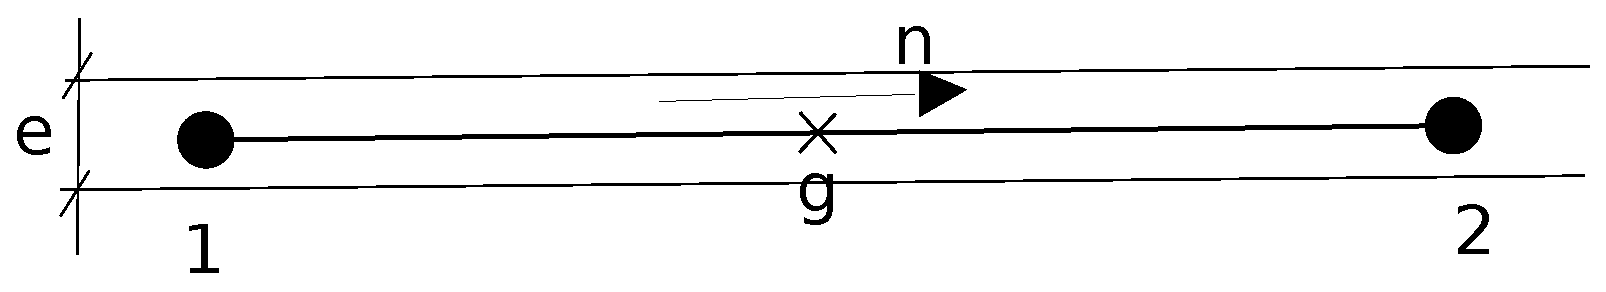
\includegraphics[width=.7\textwidth,center]{numeric-local-frac.eps} 
\caption{المان ترک و نام‌گذاری‌های محلّی}
\label{fig:3frac}
\end{figure}

\begin{tight_itemize}
\item[$e$]
ضخامت ترک. به علاوه از تعریف طول اضلاع دوگانه داریم: $l_{12} = l_{21} = e$
\item[$\vec n$]
بردار یکّه از نود ۱ به نود ۲. به علاوه از تعاریف قبلی داریم:
$\vec n = \vec n_{12} = -\vec n_{21}$ 
\item[$l$]
طول المان ترک که برابر است با
$\sqrt{ \left( x_1 - x_2 \right)^2 + \left( y_1 - y_2 \right)^2 } $
\item[$g$]
نقطه وسط المان ترک. به علاوه از تعاریف قبلی داریم:  
$g_{12} = g_{21} = g$
\end{tight_itemize}

حال توابع شکل را به صورت معادله \ref‌فر{eq:3frac1} تعریف می‌نماییم:
\begin{equation}
\label{eq:3frac1}
 \psi_1(x,y) = \frac{x-x_2}{x_1-x_2} = \frac{y-y_2}{y_1-y_2}, \quad
 \psi_2(x,y) =\frac{x-x_1}{x_2-x_1} = \frac{y-y_1}{y_2-y_1}
\end{equation}

از ترکیب معادلات \ref‌فر{eq:3sf3}،  \ref‌فر{eq:3sf4} و \ref‌فر{eq:3frac1}  نتیجه می‌شود که مقدار گرادیان پتانسیل‌ها برابر خواهد بود با:
\begin{equation}
\label{eq:3frac2}
\nabla \varphi_\alpha|_g = 
\frac{\varphi_\alpha|_2 - \varphi_\alpha|_1}{l} \vec{n} 
\qquad \alpha = w,c
\end{equation}

اکنون می‌توانیم به کمک مقادیر گرادیان پتانسیل‌ها جهت سرعت هر فاز را تعیین کرده و از روش \text‌لاتین{upwind} مقادیر
$\lambda_\alpha|_g$
را بیابیم. اگر معادلات \ref‌فر{eq:3dim4}، \ref‌فر{eq:3dim5}، \ref‌فر{eq:3up} و \ref‌فر{eq:3frac2}  را ترکیب کنیم، خواهیم داشت:
\begin{equation}
\label{eq:3frac3}
\lambda_w|_g = 
\begin{cases}
\lambda_w|_1 & \varphi_w|_1 > \varphi_w|_2 \\
\lambda_w|_2 & \text{otherwise}
\end{cases}
\quad 
\lambda_o|_g = 
\begin{cases}
\lambda_o|_1 & \varphi_w|_1 + \varphi_c|_1 > \varphi_w|_2 + \varphi_c|_2 \\
\lambda_o|_2 & \text{otherwise}
\end{cases}
\end{equation}

اکنون مقادیر 
$a_{11}$، $a_{12}$ و $b_1$
را محاسبه می‌نماییم. از معادله \ref‌فر{eq:3fvmp4}، داریم:
\begin{equation}
\label{eq:3frac4}
-\text{TFlux}_{12} = a_{11}\varphi_w|_1 + a_{11}\varphi_w|_2 + b_1
\end{equation}

از طرفی از ترکیب معادلات \ref‌فر{eq:3fvmp2} و \ref‌فر{eq:3frac2} داریم:
\begin{equation}
\label{eq:3frac5}
\begin{aligned}
-\text{TFlux}_{12} 
&= \lambda|_g K \frac{\varphi_w|_2 - \varphi_w|_1}{l} \vec{n} \cdot (e\vec n) +
\lambda_o|_g K \frac{\varphi_c|_2 - \varphi_c|_1}{l} \vec{n} \cdot (e\vec n) \\
&= -\lambda|_g\frac{Ke}{l}\varphi_w|_1 + \lambda|_g\frac{Ke}{l}\varphi_w|_1
+ \lambda_o|_g \frac{Ke}{l}(\varphi_c|_1 - \varphi_c|_2)
\end{aligned}
\end{equation}

از مقایسه \ref‌فر{eq:3frac4} و \ref‌فر{eq:3frac5} واضح است که:
\begin{equation}
\label{eq:3frac6}
a_{11} =-\lambda|_g\frac{Ke}{l}, \quad
a_{12} = \lambda|_g\frac{Ke}{l}, \quad
b_1 = \lambda_o|_g \frac{Ke}{l}(\varphi_c|_1 - \varphi_c|_2)
\end{equation}

به طریقه مشابه می‌توان دیگر مقادیر 
$a$، $b$ و مقادیر $f$
را محاسبه نمود و به ماتریس‌های محلّی زیر رسید:
\begin{equation}
\label{eq:3frac7}
\begin{aligned}
&\mathbf A =
	 \begin{bmatrix}
	-\lambda|_g\frac{Ke}{l} &\lambda|_g\frac{Ke}{l}\\
	\lambda|_g\frac{Ke}{l} &-\lambda|_g\frac{Ke}{l} 
	  \end{bmatrix} \quad
\vec{\mathcal B} = 
	\begin{bmatrix}
	\lambda_o|_g \frac{Ke}{l}(\varphi_c|_1 - \varphi_c|_2) \\
	\lambda_o|_g \frac{Ke}{l}(\varphi_c|_2 - \varphi_c|_1)
	\end{bmatrix} \\
&\vec{\mathcal F} = 
	\begin{bmatrix}
	\lambda_w|_g \frac{Ke}{l}(\varphi_w|_2 - \varphi_w|_1) \\
	\lambda_w|_g \frac{Ke}{l}(\varphi_w|_1 - \varphi_w|_2)
	\end{bmatrix}
\end{aligned}
\end{equation}

در آخر نحوه محاسبه مقادیر 
$\text{Volume}(B_i)$
را بیان می‌کنیم. در المان ترک به سادگی داریم:
\begin{equation}
\label{eq:3frac8}
\text{Volume}(B_1) = \text{Volume}(B_2) = \frac{el}{2}
\end{equation}
%--------------------------------------------ماتریس محلّی المان ماتریس------------------------------ی
\subsection{المان ماتریس}
در این قسمت نحوه محاسبه ماتریس‌های محلّی برای المان‌های دو‌بعدی را بیان خواهیم کرد (هر چند معمولاً این المان‌ها متعلق به ناحیه ماتریس هستند اگر از روش ترک-دوبعدی استفاده کنیم، می‌توانند متعلق به ناحیه ترک نیز باشند). روشی که بیان خواهیم کرد کلّی بوده و برای هر دو شکل مثلث و چهارضلعی قابل پیاده‌سازی خواهد بود. این روش از \cite{maliska-cvfem} برگرفته شده‌است. اوّل از همه برای تعریف توابع شکل از فضای مرجع $\xi \eta$ استفاده می‌کنیم. برای برقراری ارتباط بین این فضا و فضای $xy$ از یک تبدیل \text‌لاتین{isoparametric} استفاده می‌کنیم. به زبان ریاضی:
\begin{equation}
\label{eq:3poly1}
x= \sum_{i=1}^{N} x_i\psi_i(\xi,\eta), \qquad y= \sum_{i=1}^{N} y_i\psi_i(\xi,\eta)
\end{equation}

همان‌طور که در ابتدای بخش \ref{ch:36} اشاره کردیم، $ٔN$ تعداد نود‌های عضو المان مورد بحث است. در ادامه در موارد مورد نیاز $xy$ و $\xi \eta$ را با $x_1x_2$ و $\xi_1 \xi_2$ نیز نشان می‌دهیم. به علاوه منظور از $\vec \xi$ یک بردار در فضای $\xi \eta$ منظور از $\vec x$ بردار متناظر در فضای $xy$ می‌باشد. $\Omega_x$ نیز یک حجم در فضای $xy$ و $\Omega_\xi$ حجم متناظر آن در فضای  $\xi \eta$ خواهد بود.

%------x
\begin{figure}[h]
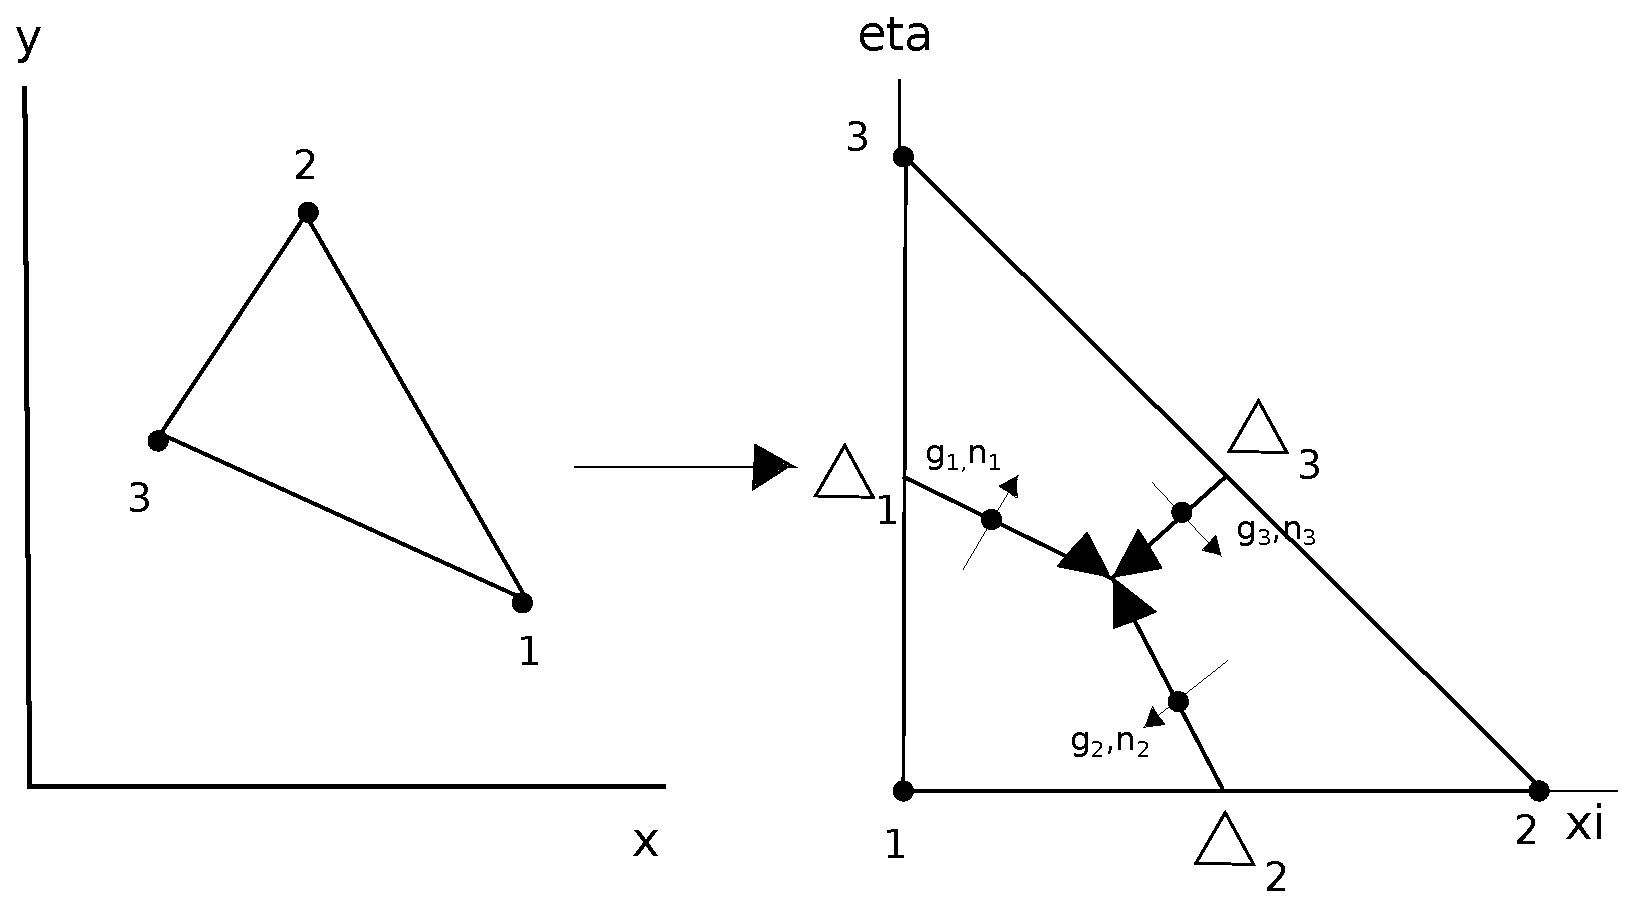
\includegraphics[width=.6\textwidth,center]{numeric-local-tri.eps} 
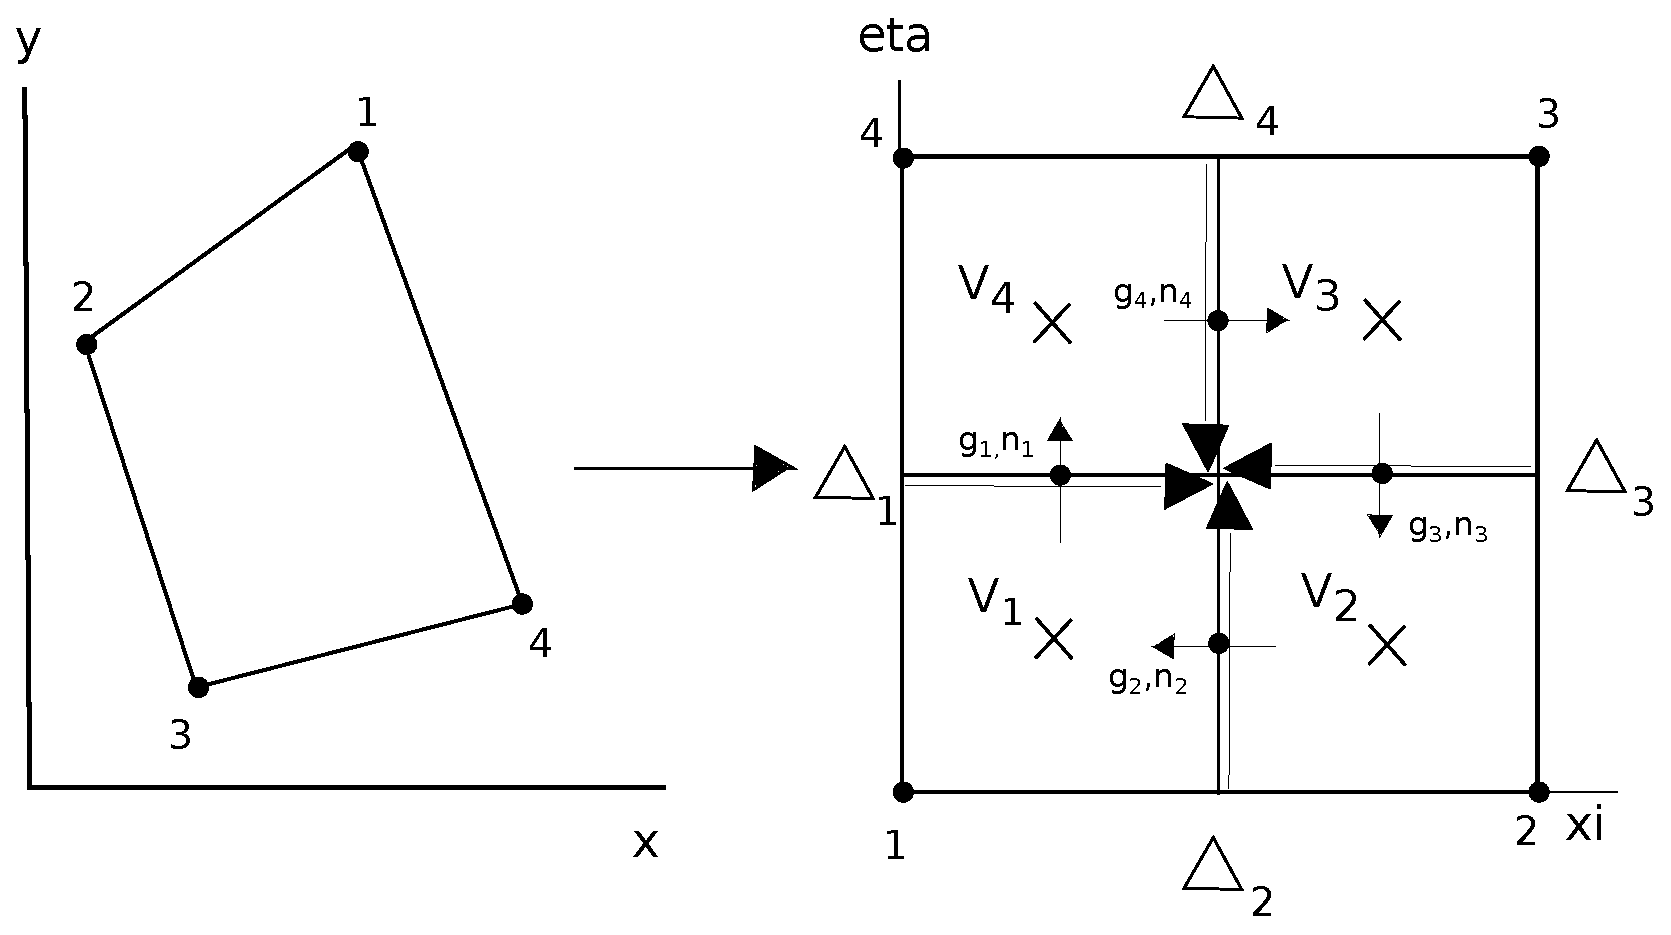
\includegraphics[width=.6\textwidth,center]{numeric-local-quad.eps} 
\caption{المان‌های مثلث و چهارضلعی و المان‌های مرجع در فضای $\xi \eta$}
\label{fig:3poly}
\end{figure}
%------x

در شکل \ref{fig:3poly} یک المان مثلث و یک المان چهارضلعی در فضای  $xy$ و المان‌های مرجع متناظرشان  در فضای  $\xi \eta$ نشان داده شده‌اند.  همانطور که مشاهده می‌کنید، مثلث مرجع یک مثلث قائم‌الزاویه و چهارضلعی مرجع یک مربع می‌باشند. مختصات رئوس آن‌ها در جدول \ref{tab:3poly} آمده است. نکته مهم این است که نام‌گذاری نود‌ها در هر دو فضا باید پادساعتگرد باشد. اکنون تعاریف جدید مورد نیاز را ارائه می‌دهیم.

%------x
\begin{table}
\centering
\caption{مختصات نود‌های اصلی، نقاط $V_i$ و بردار‌های $\vec \Delta_i$ در فضای $\xi \eta$ }
\label{tab:3poly}
\begin{tabular}{| c | c | c | c | c | c |}
\hline
ردیف &نود‌ها-چهارضلعی & نودها-مثلث &$V_i$-چهارضلعی &$\vec \Delta_i$-چهارضلعی &$\vec \Delta_i$-مثلث \\
\hline
۱ &$0,0$ &$0,0$ &$^1/_4,^1/_4$ &$^1/_2,0$    &$^1/_3,^{-1}/_6$   \\
۲ &$1,0$ &$1,0$ &$^3/_4,^1/_4$ &$0,^1/_2$    &$^{-1}/_6,^1/_3$   \\
۳ &$1,1$ &$0,1$ &$^3/_4,^3/_4$ &$^{-1}/_2,0$ &$^{-1}/_6,^{-1}/_6$ \\
۴ &$0,1$ &-- &$^1/_4,^3/_4$ &$0,^{-1}/_2$ &-- \\
\hline
\end{tabular}
\end{table}
%------x

\subsection*{نقاط انتگرال‌گیری حجم}
نقطه مرکز هندسی زیر حجم کنترل $B_i$ در فضای $\xi \eta$ را نقطه انتگرال‌گیری حجم یا $V_i$ می‌نامیم. مختصات این نقطه در المان‌های چهارضلعی برای محاسبه حجم $B_i$ استفاده می‌شوند ولی در المان‌های مثلثی نیازی به آن‌ها نیست. مختصات این نقاط برای المان مرجع مربع در جدول\ref{tab:3poly} آمده‌ است.

\subsection*{ماتریس توابع شکل}
ماتریس  توابع شکل
 $ \mathbf{\Psi}_{1 \times N} $
  را به صورت 
$\left[ \psi_1 \quad \ldots \quad \psi_N \right]$
تعریف می‌کنیم. این ماتریس برای المان‌ها به صورت معادله \ref‌فر{eq:3poly2} خواهد بود.
\begin{equation}
\label{eq:3poly2}
\begin{aligned}
\text{quad}: \quad  \mathbf \Psi &{}= 
	\begin{bmatrix}
	1-\xi-\eta &\xi &\eta
	\end{bmatrix} \\
\text{triangle}: \quad  \mathbf \Psi &{}=
	\begin{bmatrix}
	(1-\xi)(1-\eta) &\xi(1-\eta) &\xi\eta &(1-\xi)\eta 
	\end{bmatrix} 
\end{aligned}
\end{equation}

\subsection*{ماتریس مشتق توابع شکل}
ماتریس مشتق توابع شکل یا 
$\frac{\partial \mathbf \Psi}{\partial \vec \xi}$
به صورت معادله تعریف می‌شود:
\begin{equation}
\label{eq:3poly3}
\frac{\partial \mathbf \Psi}{\partial \vec \xi} = 
\left[ \frac{\partial \psi_i}{\partial \xi_j} \right]_{N \times 2} 
\quad i = 1,\ldots,N \quad j=1,2
\end{equation}

اگر معادله \ref‌فر{eq:3poly2} را در معادله \ref‌فر{eq:3poly3} جایگذاری کنیم، ماتریس مشتق توابع شکل برای المان‌های مثلث و چهار‌ضلعی به دست می‌آید:
\begin{equation}
\label{eq:3poly4}
\left. \frac{\partial \mathbf \Psi}{\partial \vec \xi} \right)_{triangle} = 
	\begin{bmatrix}
	-1 &-1 \\ 1 &0 \\ 0 &1 
	\end{bmatrix} 
\qquad  \left. \frac{\partial \mathbf \Psi}{\partial \vec \xi} \right)_{quad}  =
	\begin{bmatrix}
	-(1-\eta) &-(1-\xi) \\ 1-\eta &-\xi \\ \eta &\xi \\ -\eta &1-\xi
	\end{bmatrix} 
\end{equation}

\subsection*{ماتریس مختصات}
مختصات همه نقاط را داخل یک ماتریس قرار داده و آن را ماتریس مختصات می‌نامیم و با $\mathbf X$ نمایش می‌دهیم. به زبان ریاضی:
\begin{equation}
\label{eq:3poly5}
\mathbf X = 
	\begin{bmatrix}
	x_1 &\ldots &x_N \\ y_1 &\ldots &y_N
	\end{bmatrix} 
\end{equation}
\subsection*{ماتریس یاکوبی}
ماتریس یاکوبی به صورت زیر تعریف می‌شود:
\begin{equation}
\label{eq:3poly6}
\textbf J = 
\left[ \frac{\partial x_i}{\partial \xi_j} \right]_{2 \times 2} \quad i,j = 1,2
\end{equation}

این ماتریس سه خاصیت بسیار مهم دارد که از آن‌ها استفاده خواهیم کرد:
\begin{align}
\label{eq:3poly7}
&d\Omega_x = \text{det}(\textbf J) d\Omega_\xi \\
\label{eq:3poly7x}
&d\vec x = \textbf J d\vec \xi \\
\label{eq:3poly7xx}
&\left( \nabla_x \varphi_\alpha \right)^T = \left(\nabla_\xi \varphi_\alpha\right)^T \textbf J ^ {-1}
\end{align}

با ترکیب معادلات \ref‌فر{eq:3poly1}، \ref‌فر{eq:3poly2} و استفاده از قاعده زنجیره‌ای می‌توان نشان داد که ماتریس یاکوبی را می‌توان از معادله زیر محاسبه کرد:
\begin{equation}
\label{eq:3poly8}
\textbf J =  \textbf X \frac{\partial \mathbf \Psi}{\partial \vec \xi} 
\end{equation}

\subsection*{پارامتر‌های مربوط به اضلاع دوگانه}
مقادیر 
$\vec n_i$ ، $g_i$ و $l_i$
به ترتیب متناظر بردار یکّه نرمال، نقطه وسط و طول اضلاع دوگانه داخل المان هستند. نحوه نام‌گذاری اضلاع دوگانه و جهت بردار‌های $\vec n_i$ در شکل \ref{fig:3poly} نشان داده شده‌است. برای مثال برای المان مثلث رابطه بردارهای $\vec n_i$ و $\vec n_{ij}$ به صورت 
$\vec n_1 = \vec n_{13}$ ، $\vec n_2 = \vec n_{21}$ و $\vec n_3 = \vec n_{32}$
می‌باشد.

\subsection*{بردارهای $\vec \Delta$}
در فضای $\xi \eta$ بردار‌ $\vec \Delta$ را برداری تعریف می‌کنیم که هم‌راستا با ضلع دوگانه‌ای است که نقطه وسط آن $g_i$ باشد و جهت آن به سمت داخل المان باشد. در شکل \ref{fig:3poly} راستا و جهت و در جدول \ref{tab:3poly} مختصات این بردار‌ها برای المان‌های مرجع مثلث و مربع نشان داده‌ شده‌اند. از رابطه \ref‌فر{eq:3poly7x} می‌توان ثابت کرد:
\begin{equation}
\label{eq:3poly9}
l_i\vec n_i = \textbf R \textbf J \vec \Delta_i, 
\qquad \textbf{R} = 
	\begin{bmatrix}
	0 &-1 \\ 1 &0 
	\end{bmatrix} \quad
\end{equation}

در این رابطه $\textbf R$ ماتریس دوران ۹۰ درجه در راستای خلاف عقربه‌های ساعت است.

\subsection*{بردار مقادیر محلّی}
مقادیر محلّی $\varphi_\alpha$ را در یک بردار قرار داده و آن را بردار مقادیر المان می‌نامیم. به زبان ریاضی:
\begin{equation}
\label{eq:3poly10}
\vec \varphi_\alpha = 
	\begin{bmatrix}
	\varphi_\alpha|_1 &\ldots &\varphi_\alpha|_N 
	\end{bmatrix}^T \quad
\alpha = w,o
\end{equation}
\subsection*{ماتریس‌ شار}
برای هر المان  ماتریس شار  $\textbf {H}_{N\times N}$  را ماتریسی تعریف می‌کنیم که در رابطه زیر صدق کند ($\textbf H_i$ یعنی سطر $i$ام $\textbf H$):
\begin{equation}
\label{eq:3poly11}
\textbf H_i \vec \varphi_\alpha = \textbf K \nabla \varphi_\alpha|_{g_i} \cdot l_i\vec n_i
\qquad i = 1,\ldots,N
\end{equation}

با استفاده از روابط \ref‌فر{eq:3poly9} و \ref‌فر{eq:3poly7xx} می‌توان ثابت کرد که ماتریس $\textbf H_i$ را می‌توان از رابطه زیر محاسبه کرد:
\begin{equation}
\label{eq:3poly12}
\textbf H_i = \left( 
\left. \frac{\partial \mathbf \Psi}{\partial \vec \xi} \right|_{g_i} 
 \textbf J^{-1}|_{g_i} \textbf K^T \textbf R  \textbf J|_{g_i} \vec \Delta_i
 \right)^T
\qquad i = 1,\ldots,N
\end{equation}

با کمک تعاریفی که ارائه دادیم می‌توانیم محاسبه ماتریس‌های محلّی را شروع کنیم. ابتدا نحوه محاسبه مقادیر \text‌لاتین{upwind} را نشان می‌دهیم. با استفاده از روابط \ref‌فر{eq:3up} و \ref‌فر{eq:3poly11} می‌توان نشان داد که مقادیر $\lambda|_{g_i}$ را  می‌توان از روابط زیر محاسبه نمود:
\begin{equation}
\label{eq:3poly13}
\lambda_w|_{g_i} = 
	\begin{cases}
	\lambda_w|_i &-\textbf H_i \vec \varphi_w > 0 \\	
	\lambda_w|_{i-1} &-\textbf H_i \vec \varphi_w < 0 \& i \geq 2 \\	
	\lambda_w|_N &-\textbf H_i \vec \varphi_w < 0 	\& i = 1	
	\end{cases} \quad
\lambda_o|_{g_i} = 
	\begin{cases}
	\lambda_o|_i &-\textbf H_i  (\vec \varphi_o + \vec \varphi_w) > 0 \\	
	\lambda_o|_{i-1} &-\textbf H_i  (\vec \varphi_o + \vec \varphi_w)<0 \& i \geq 2 \\	
	\lambda_o|_N &-\textbf H_i  (\vec \varphi_o + \vec \varphi_w)<0	\& i = 1	
	\end{cases}
\end{equation}

اکنون نحوه محاسبه مقادیر $a$ و $b$ را برای نود شماره ۱ نشان می‌دهیم. به این منظور از رابطه \ref‌فر{eq:3fvmp4} داریم:
\begin{equation}
\label{eq:3poly14}
\sum_{j=2,4} -\text{TFlux}_{1j} = 
\begin{bmatrix}
	a_{11} &\ldots &a_{1N} 
\end{bmatrix}
\begin{bmatrix}
	\varphi_w|_1 \\ \vdots \\ \varphi_w|_N
\end{bmatrix}
+ b_1
\end{equation}

از طرفی از ترکیب معادلات  \ref‌فر{eq:3fvmp2}  داریم :
\begin{equation}
\label{eq:3poly15}
\begin{aligned}
\sum_{j=2,4} -\text{TFlux}_{1j} = 
&+\lambda|_{g_1} \textbf K \nabla \varphi_w|_{g_1} \cdot (l\vec n)_1 
&+\lambda_o|_{g_1} \textbf K \nabla \varphi_c|_{g_1} \cdot (l\vec n)_1 \\
&-\lambda|_{g_2} \textbf K \nabla \varphi_w|_{g_2} \cdot (l\vec n)_2 
&-\lambda_o|_{g_2} \textbf K \nabla \varphi_c|_{g_2} \cdot (l\vec n)_2 \\
\end{aligned} 
\end{equation}

حال با ترکیب \ref‌فر{eq:3poly15} و  \ref‌فر{eq:3poly11} داریم:
\begin{equation}
\label{eq:3poly16}
\sum_{j=2,4} -\text{TFlux}_{1j} = 
\left( \lambda|_{g_1} \textbf H_1 - \lambda|_{g_2} \textbf H_2 \right)
\begin{bmatrix}
	\varphi_w|_1 \\ \vdots \\ \varphi_w|_N
\end{bmatrix}
+
\left( \lambda_o|_{g_1} \textbf H_1 - \lambda_o|_{g_2} \textbf H_2 \right)
\begin{bmatrix}
	\varphi_c|_1 \\ \vdots \\ \varphi_c|_N
\end{bmatrix}
\end{equation}

از مقایسه دو معادله \ref‌فر{eq:3poly14} و  \ref‌فر{eq:3poly16} مقادیر $a$ و $b$ را برای نود شماره ۱ به دست می‌آید:
\begin{equation}
\label{eq:3poly17}
\begin{bmatrix}
	a_{11} &\ldots &a_{1N} 
\end{bmatrix} 
=  \left( \lambda|_{g_1} \textbf H_1 - \lambda|_{g_2} \textbf H_2 \right) , \quad 
b_1 = 
\left( \lambda_o|_{g_1} \textbf H_1 - \lambda_o|_{g_2} \textbf H_2 \right)
\begin{bmatrix}
	\varphi_c|_1 \\ \vdots \\ \varphi_c|_N
\end{bmatrix}
\end{equation}

به طریقه مشابه می‌توان دیگر مقادیر
 $a$، $b$ و $f$
را محاسبه کرد و ماتریس‌ $\textbf A$ و بردار‌های $\vec{\mathcal B}$ و $\vec{\mathcal F}$ را به صورت زیر به دست آورد:
\begin{equation}
\label{eq:3poly18}
\begin{aligned}
&\textbf A =
\begin{bmatrix}
	\lambda|_{g_1} \textbf H_1 - \lambda|_{g_2} \textbf H_2 \\
	\vdots \\ 
	\lambda|_{g_{N-1}} \textbf H_{N-1} - \lambda|_{g_{N}} \textbf H_N \\
	\lambda|_{g_N} \textbf H_N - \lambda|_{g_1} \textbf H_1
\end{bmatrix}
\vec {\mathcal B} = 
\begin{bmatrix}
	-\left( \lambda_o|_{g_1} \textbf H_1 - \lambda_o|_{g_2} \textbf H_2 \right) \vec \varphi_c \\
	 \vdots  \\ 
	-\left( \lambda_o|_{g_{N-1}} \textbf H_{N-1}- \lambda_o|_{g_{N}} \textbf H_N \right) \vec \varphi_c \\
	-\left( \lambda_o|_{g_N} \textbf H_N - \lambda_o|_{g_1} \textbf H_1  \right) \vec \varphi_c
\end{bmatrix} \\
&\vec {\mathcal F} = 
\begin{bmatrix}
	\left( \lambda_w|_{g_1} \textbf H_1 - \lambda_w|_{g_2} \textbf H_2 \right) \vec \varphi_w \\
	 \vdots  \\ 
	\left( \lambda_w|_{g_{N-1}} \textbf H_{N-1}- \lambda_w|_{g_{N}} \textbf H_N \right) \vec \varphi_w \\
	\left( \lambda_w|_{g_N} \textbf H_N - \lambda_w|_{g_1} \textbf H_1  \right) \vec \varphi_w
\end{bmatrix} 
\end{aligned}
\end{equation}

در آخر نحوه محاسبه حجم $B_i$ها را ذکر می‌کنیم. با استفاده از رابطه \ref‌فر{eq:3poly7} تقریب مقدار میانی برای محاسبه انتگرال‌ها می‌توانیم بنویسیم:
\begin{equation}
\label{eq:3poly19}
\text{Volume}(B_i) = \int_{B_i}d\Omega_x = \int_{B_i}\text{det}(\textbf J)d\Omega_\xi \approx
\begin{cases}
\frac{1}{4}\text{det}(\textbf J)|_{V_i} &\text{quad} \\
\frac{1}{6}\text{det}(\textbf J) &\text{triangle}
\end{cases}
\end{equation}

در مثلث‌ها ماتریس یاکوبی تابعی از مکان نیست، امّا در المان‌های چهارضلعی دترمینان این ماتریس باید در نقاط انتگرال‌گیری حجم محاسبه شود.

%--------------------------------------------ماتریس محلّی المان شرایط مرزی------------------------------ی
\subsection{المان شرایط مرزی}
\begin{figure}
\begin{subfigure}{.5\textwidth}
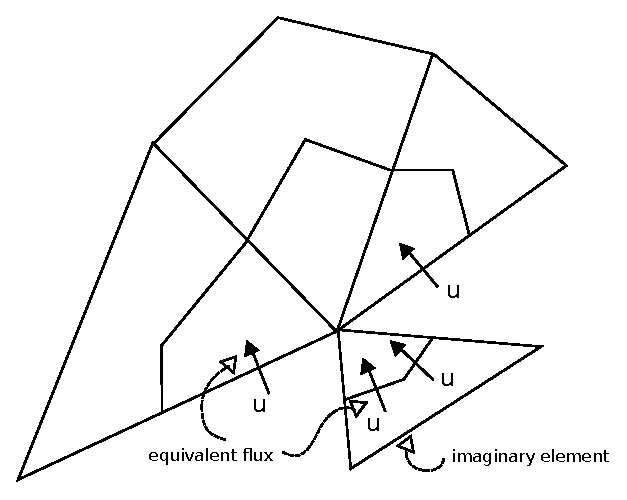
\includegraphics[width=.9\linewidth,center]{numeric-bnd-flux.eps} 
\caption{فرض می‌شود شار ورودی به حجم کنترل از یک المان فرضی وارد آن می‌شود}
\label{fig:3bnd-imaj}
\end{subfigure}
\begin{subfigure}{0.5\textwidth}
\includegraphics[width=.9\linewidth,center]{numeric-bnd-notation.eps} 
\caption{نام‌گذاری نودها و حجم کنترل}
\label{fig:3bnd-real}
\end{subfigure}
\caption{یک نود روی مرز هندسه}
\label{fig:3bnd}
\end{figure}

شکل \ref{fig:3bnd-real} یک نود که روی مرز قرار دارد و حجم کنترل متناظرش را نمایش می‌دهد. نام این نود $i$ و نام نود‌های مجاورش که روی مرز قرار دارند $j$ و $k$ می‌باشد. به علاوه نیمی از ضلع $ij$ به ناحیه مرزی $\Gamma_1$ و نیمی  از ضلع $ik$ به ناحیه مرزی $\Gamma_2$ تعلق دارد. هدف ما این است که شاری که از اضلاع $ij$ و $ik$ وارد حجم کنترل می‌شوند را محاسبه کنیم و تعیین کنیم که وجود این شار‌ها چه تغییراتی در
 $\textbf A_G$، $\vec{\mathcal B}_G$ و $\vec{\mathcal F}_G$
ایجاد می‌کنند. به علاوه  این شار‌ها نشان می‌دهند که در هر گام زمانی چه مقدار سیال به مخزن وارد یا از مخزن خارج شده است. حالات زیر را در نظر بگیرید:
\begin{tight_enumerate}
\item در هر دو ناحیه مرزی $\Gamma_1$ و $\Gamma_2$ شرط مرزی نفوذناپذیر حاکم باشد. در این حالت هیچ شاری از $ij$ و $ik$ عبور نمی‌کند. لذا این نود تأثیری در $\textbf A_G$، $\vec{\mathcal B}_G$ و $\vec{\mathcal F}_G$ و یا سیال ورودی و خروجی به مخزن نخواهد داشت.

\item در نواحی $\Gamma_1$ و $\Gamma_2$ دو شرط مرزی نفوذپذیر و متفاوت حاکم باشد. روش عددی ما قادر به مدل کردن چنین حالتی نیست. لذا در صورت بروز چنین حالتی بهتر است یک ناحیه کوچک نفوذناپذیر بین دو ناحیه $\Gamma_1$ و $\Gamma_2$ ایجاد کنیم.

\item $\Gamma_1$ نفوذپذیر باشد و $\Gamma_2$ یا نفوذناپذیر باشد یا همان $\Gamma_1$ باشد. از بین حالات عنوان شده این حالت است که نیاز به اعمال تدابیر ویژه‌ای دارد و در ادامه فقط لازم است به این حالت بپردازیم.
\end{tight_enumerate}

با توجه به فرضیات عنوان شده در حالت سوم، بردار مرزی نود $i$ یا همان $(ln)_i$ را به صورت معادله \ref‌فر{eq:3bnd1} تعریف می‌کنیم.
\begin{equation}
\label{eq:3bnd1}
(l\vec n)_i = \begin{cases}
\frac{1}{2} \left( \text{length}(ij)\vec n_{ij} + \text{length}(ik)\vec n_{ik} \right) \quad &\Gamma_1 = \Gamma_2 \\
\frac{1}{2} \text{length}(ij)\vec n_{ij} \quad &\Gamma_2 = \text{impermeable} 
\end{cases}
\end{equation}

در این معادله بردار‌های $\vec n$ بردارهای یکّه عمود بر ضلع متناظر به سمت خارج مرز هستند. به علاوه $l_i$ را برابر طول $\partial B_i \bigcap \Gamma_1$ تعریف می‌کنیم. میزان شار آب و کل عبوری از 
$\partial B_i \bigcap \Gamma_1$  را به ترتیب با $u_{w\Gamma i}$ و $u_{\Gamma i}$
نشان می‌دهیم. مطابق شکل  \ref{fig:3bnd-imaj} می‌توانیم فرض کنیم این شار از یک المان مجازی وارد $B_i$ می‌شود.اگر این المان را $e_{bnd}$ بنامیم، با توجه به معادلات \eqref{eq:3fvmp4} و \eqref{eq:3fvms3} داریم:

\begin{equation}
\label{eq:3bnd2}
\begin{aligned}
u_{w\Gamma_i}= \sum_{v_j \in \eta(v_i,e_{bnd})} -\frac{1}{\mathcal P}\text{SFlux}_{ij}^{bnd} = 
\frac{1}{\mathcal P}f_i^{bnd} \\
u_{\Gamma_i} = \sum_{v_j \in \eta(v_i,e_{bnd})} -\frac{1}{\mathcal P}\text{TFlux}_{ij}^{bnd} = 
\frac{1}{\mathcal P}b_i^{bnd}
\end{aligned}
\end{equation}

دقت کنید که برای المان فرضی $e_{bnd}$ مقادیر $a_{ij}$ برابر صفر هستند. حال به کمک معادلات \eqref{eq:3fvmp10} و \eqref{eq:3fvms9} می‌توانیم شروط مرزی را با اسمبل کردن بردار‌های محلّی المان‌ $e_{bnd}$ اعمال کنیم. نحوه انجام این کار را برای هر نوع شرط مرزی به صورت جداگانه بیان خواهیم کرد.

\subsection*{شرط مرزی نیومن برای پتانسیل}
در این حالت چون مقدار سرعت روی مرز داده شده است (رجوع شود به معادله  \eqref{eq:2bndout} ) ابتدا می‌توانیم مقدار $u_{\Gamma i}$ را محاسبه کنیم:
\begin{equation}
\label{eq:3bnd3}
u_{\Gamma_i}= -u_N l_i
\end{equation}

وجود علامت منفی به این خاطر است که $u_N$ مؤلفه سرعت به سمت خارج مرز را نشان می‌دهد امّا $u_{\Gamma_i}$ شار ورودی را نشان می‌دهد. لذا از معادله  \eqref{eq:3bnd2} بردار محلّی المان فرضی که تنها عضوش نود $v_i$ است، برابر است با:
\begin{equation}
\label{eq:3bnd4}
\vec{\mathcal B} = 
	\begin{bmatrix}
	- \mathcal P u_{\Gamma_i}
	\end{bmatrix}
\end{equation}
\subsection*{شرط مرزی دیریشله برای پتانسیل}
در این حالت مقدار
$\varphi_w|_{vi} = \varphi_{D}$
را با قرار دادن  $\vec {\mathcal B}_{Gi}$ برابر $\varphi_D$ و برابر کردن سطر $i$اُم  ماتریس $\textbf A_G$ با ماتریس همانی، به دستگاه  \eqref{eq:3impes1} اعمال می‌کنیم. برای محاسبه $u_{\Gamma i}$ بعد از حل دستگاه  \eqref{eq:3impes1}، فرض کنید که جواب دستگاه برابر $\vec \Phi$ و 
$\mathcal B_{Gi}$ و $\textbf A_{Gi}$
به ترتیب برابر درایه و سطر $i$اُم $\vec {\mathcal B}_{G}$ و $\textbf A_G$ قبل از اعمال شرط مرزی باشند. آن گاه می‌توانیم بنویسیم:
\begin{equation}
\label{eq:3bnd5}
u_{\Gamma_i}= \frac{1}{\mathcal P} \left( \mathcal B_{Gi} - \textbf A_{Gi} \vec \Phi \right)
\end{equation}

\subsection*{شرط مرزی نیومن برای اشباع}
در این حالت مقدار $u_{\Gamma i}$ از قبل توسط یکی از معادلات \eqref{eq:3bnd3} یا \eqref{eq:3bnd3} محاسبه شده است. حال برای محاسبه $u_{w\Gamma i}$ از ترکیب  \ref‌فر{eq:3dim4}، \ref‌فر{eq:3dim5} و \ref‌فر{eq:2bndout} می‌توان نوشت:
\begin{equation}
\label{eq:3bnd6}
u_{w\Gamma_i}= \left( u_{\Gamma_i} - 
\frac{1}{\mathcal P}  \lambda_o|_{d^*_i} \mathcal G \textbf K \nabla h \cdot (l\vec n)_i  \right) 
\times \frac{\lambda_w|_{d^*_i}}{\lambda|_{d^*_i}}
\end{equation}

در این معادله \lr{\textbf{K}} تراوایی مطلق المان‌هایی است که $v_i$ عضو آن‌هاست. سپس بردار محلّی المان فرضی برابر خواهد بود با:
\begin{equation}
\label{eq:3bnd7}
\vec{\mathcal F} = 
	\begin{bmatrix}
	\mathcal P u_{w\Gamma_i}
	\end{bmatrix}
\end{equation}

\subsection*{شرط مرزی دیریشله برای اشباع}
در این حالت مقدار $\triangle S_i = 0$ را به دستگاه \eqref{eq:3impes2} با صفر کردن درایه $i$اُم $\vec {\mathcal F_{G}}$  اعمال می‌کنیم. یعنی:
\begin{equation}
\label{eq:3bnd8}
\mathcal F_{Gi} = 0
\end{equation} 

سپس برای محاسبه $u_{w\Gamma i}$ اگر $\mathcal F_{Gi} $ درایه $i$اُم $\vec {\mathcal F_{G}}$ قبل از صفر کردن باشد می‌نویسیم:
\begin{equation}
\label{eq:3bnd9}
u_{w\Gamma_i}= \frac{1}{\mathcal P} \mathcal F_{Gi} 
\end{equation}
\subsection*{محاسبه میزان سیال ورودی به و خروجی از مخزن}
فرض کنید 
$Q^k_{w,in}$، $Q^k_{w,out}$، $Q^k_{in}$  و $Q^k_{out}$
به ترتیب برابر میزان آب ورودی، میزان آب خروجی، کل سیال ورودی و کل سیال خروجی از آغاز تا گام زمانی $k$ به مخزن باشند. می‌توان نوشت:
\begin{equation}
\begin{aligned}
\label{eq:3bnd10}
&Q^{k+1}_{w,in} = &Q^k_{w,in} &+ \triangle t\sum max(u_{w\Gamma} , 0) \\
&Q^{k+1}_{w,out} = &Q^k_{w,out} &-\triangle t\sum min(u_{w\Gamma} , 0) \\
&Q^{k+1}_{in} = &Q^k_{in} &+\triangle t\sum max(u_{\Gamma} , 0) \\
&Q^{k+1}_{out} = &Q^k_{out} &-\triangle t\sum min(u_{\Gamma} , 0)
\end{aligned}
\end{equation}
در این معادله اپراتور جمع باید بر روی تمامی نود‌هایی که روی مرز قرار دارند اعمال شود.

%----------------------------------------------------------------------------------------ی
%----------------------------------------------------------------------------------------ی
%                                      قسمت پنجم: گام زمانی
%----------------------------------------------------------------------------------------ی
%----------------------------------------------------------------------------------------ی
\section{انتخاب گام زمانی}
روش \text‌لاتین{IMPES} بسیار حساس به گام زمانی است و در صورتی که گام زمانی بیش از حد بزرگ شود، پاسخ‌ها واگرا خواهند شد. لذا از الگوریتم \ref{alg:alg1} برای محاسبه گام زمانی استفاده می‌کنیم \cite{mont1}. در این این پروژه معمولاً مقادیر $0.01$، $0.005$ و $1.2$ برای مقادیر
 $\triangle S_{max}$،   $\triangle S_{min}$ و $\beta$
در نظر گرفته شده‌اند.

\begin{algorithm}      
	\small
\caption{انتخاب گام زمانی $\triangle t$}  
\label{alg:alg1}                 
\begin{algorithmic}[1]	
	\REQUIRE $\vec{\mathcal C}$، $\vec{\mathcal F}$، حدس اوّلیه برای $\triangle t$، 
		$\triangle S_{max}$، $\triangle S_{min}$، $\beta$، $\triangle t_{max}$ و $\triangle t_{min}$.       			
	\ENSURE $\triangle \vec{S}$ و $ \triangle t$
	\STATE $\triangle \vec S$ را از معادله \eqref{eq:3impes2} با استفاده از حدس اوّلیه برای  $\triangle t$  محاسبه کن.
	\STATE محاسبه کن: $x= \Vert \triangle \vec S \Vert_\infty$
	\IF {$x < \triangle S_{min}$} 
		\STATE جواب را قبول کن و برای گام زمانی بعدی قرار بده: $\triangle t = min(\beta \triangle t, \triangle t_{max})$. 
	\ELSIF {$\triangle S_{min} < x < \triangle S_{max}$}
		\STATE پاسخ را قبول کن و تغییری در  $\triangle t$ ایجاد نکن.
	\ELSIF {$\triangle t / \beta > \triangle t_{min}$} 
		\STATE قرار بده: $\triangle t = \triangle t / \beta$ و به مرحله ۱ برگرد.
	\ELSE
		\STATE پیام خطا چاپ کن و پروسه شبیه‌سازی را متوقف کن. 
	\ENDIF
\end{algorithmic}      
\end{algorithm}

%----------------------------------------------------------------------------------------ی
%----------------------------------------------------------------------------------------ی
%                                      قسمت ششم: جمع بندی
%----------------------------------------------------------------------------------------ی
%----------------------------------------------------------------------------------------ی
\section{جمع‌بندی}
در این فصل در ابتدا معادلات حاکم بر مسئله را به حالت بدون بعد در آوردیم و نشان دادیم که پارامتر‌های بدون بعد حاکم بر مسئله مانند معادله \ref‌فر{eq:3dim7} می‌باشند. پس از آن به بررسی شبکه محاسباتی پرداختیم و تعاریف مورد نیاز مربوط به آن را ارائه دادیم. در ادامه روش‌های \text‌لاتین{IMPES} و حجم محدود معرفی و نحوه استفاده از آن‌ها برای حل مسئله بیان شد. در این قسمت روش عددی خود را در الگوریتم \ref{alg:alg2} خلاصه می‌نماییم. این الگوریتم در قالب یک کد به زبان \text‌لاتین{C++} پیاده‌سازی شده است. 

برای پیاده‌سازی کد محاسباتی از کتابخا‌نه‌ها و برنامه‌های متن‌باز مختلفی استفاده شده‌است. برای تولید شبکه محاسباتی از نرم‌افزار‌های \text‌لاتین{Gmsh}\cite{gmsh} و \text‌لاتین{Triangle}\cite{triangle} استفاده شده است. برای حل دستگاه معادلات \ref‌فر{eq:3impes1} و ذخیره ماتریس‌های اسپارس از کتابخانه \text‌لاتین{Petsc}\cite{petsc1,petsc2} بهره گرفته‌ شده‌است. این کتابخانه ابزارهای مناسبی برای رفع اشکال کد را نیز در اختیار مؤلف قرار داده‌است. جبر ماتریسی مورد نیاز برای محاسبه ماتریس‌های محلّی المان‌های مثلثی و چهار‌ضلعی به کمک کتابخانه \text‌لاتین{Armadillo}\cite{arma} برنامه‌نویسی شده است. درآخر نرم‌افزارهای \text‌لاتین{Paraview}\cite{paraview}، \text‌لاتین{Octave}\cite{octave} و \text‌لاتین{VisIt}\cite{visit} ابزار مناسب برای رسم گرافیکی پاسخ‌های آمده در فصل \ref{ch:fasl4} را فراهم کردند.

\begin{algorithm}
	\small    
\caption{خلاصه روش عددی}   
\label{alg:alg2}  
\begin{algorithmic}[1]      
	\REQUIRE .
	\\ هندسه مسئله 
	\\ شبکه محاسباتی 
	\\ شرایط مرزی مطابق معادله \ref‌فر{eq:2bndout} 
	\\ شرایط اوّلیه مطابق معادله \ref‌فر{eq:2ini} 
	\\ اعداد بی بعد مطابق معادله \ref‌فر{eq:3dim7} و جهت جاذبه : $\nabla h$ 
	\\ ویژگی‌های هر ناحیه سنگ مخزن: $\textbf{K}$، $\phi$، $P_d$، $k_{rw}$، $k_{ro}$ و ضخامت نواحی ترک: $e$
	\\ منحنی‌ فشار مویینگی: $J$
	\\ پارامتر‌های کنترل گام زمانی مطابق الگوریتم \ref{alg:alg1}
	\\ زمان اتمام شبیه‌سازی: $t_{final}$ 
	\ENSURE $\vec{\Phi}$، $\vec{S}$ و میزان سیال خروجی از و ورودی به مخزن در  $t=t_{final}$
	\STATE قرار بده $t=0$, $Q^k_{w,in}=Q^k_{w,out}=Q^k_{in}=Q^k_{out}=0$ و $\vec{\Phi} = \vec{0}$
	\STATE مقدار  $(ln)$ را برای نودهایی که روی مرز قرار دارند، مطابق معادله \eqref{eq:3bnd1} محاسبه کن.
	\STATE مقدار $u_{\Gamma i}$ را برای نود‌هایی که روی مرز $\Gamma_{\varphi N}$: قرار دارند، مطابق معادله \eqref{eq:3bnd3} محاسبه کن.
	\STATE ماتریس $\textbf H$ را برای تمام المان‌های چهارضلعی و مثلثی، مطابق معادله  (\ref{eq:3poly12}) محاسبه کن.
	\WHILE {$t < t_{final}$}
		\STATE مقادیر $\lambda_\alpha|_{gـi}$ را از معادلات   \eqref{eq:3frac3} و \eqref{eq:3poly13} محاسبه کن.
		\STATE $\textbf A_G$ و $\vec{\mathcal B}_G$ را به کمک ماتریس‌های محلّی در معادلات \eqref{eq:3frac7} و \eqref{eq:3poly18} اسمبل کن.
		\STATE شرایط مرزی $\Gamma_\varphi$ را بر روی $\textbf A_G$ و $\vec{\mathcal B}_G$ از معادله \eqref{eq:3bnd4} اعمال کن. 
		\STATE معادله \eqref{eq:3impes1} را حل کن و  $\vec \Phi$ را پیدا کن.
		\STATE مقادیر $u_{\Gamma i}$ را برای نودهای روی مرز $\Gamma_{\varphi D}$ مطابق معادله \eqref{eq:3bnd5} محاسبه کن.
		\STATE  مقادیر $\lambda_\alpha|_{gـi}$ را دوباره محاسبه کن.
		\STATE بردارهای $\vec{\mathcal F}_G$ و $\vec{\mathcal C}_G$ را از معادلات \eqref{eq:3frac7}، \eqref{eq:3poly18} و \eqref{eq:3fvms9} محاسبه کن.
		\STATE مقادیر $u_{w\Gamma i}$  را از معادلات  \eqref{eq:3bnd9} و \eqref{eq:3bnd6} محاسبه کن.
		\STATE شرایط مرزی $\Gamma_S$ را بر روی $\vec{\mathcal F}_G$ مطابق معادلات \eqref{eq:3bnd8} و \eqref{eq:3bnd7} اعمال کن. 
		\STATE معادله \eqref{eq:3impes2} را با استفاده از گام زمانی مناسب، مطابق الگوریتم \ref{alg:alg1} حل کن.
		\STATE مقادیر سیال تزریقی و برداشتی را از معادله \eqref{eq:3bnd10} به روز‌رسانی کن.
		\STATE قرار بده: $t=t+\triangle t$
	\ENDWHILE	
	\RETURN $\vec{\Phi}$، $\vec{S}$، $Q_{w,in}$، $Q_{w,out}$، $Q_{in}$ و $Q_{out}$. 
\end{algorithmic}    
\end{algorithm}
